% arara: indent: {overwrite: yes}
% options:
% thesis=B bachelor's thesis
% thesis=M master's thesis
% czech thesis in Czech language
% slovak thesis in Slovak language
% english thesis in English language
% hidelinks remove colour boxes around hyperlinks

\documentclass[thesis=B,czech]{resources/FITthesis}[2012/06/26]

\usepackage[utf8]{inputenc} % LaTeX source encoded as UTF-8

\usepackage{graphicx} %graphics files inclusion
\usepackage{listings}
\usepackage{color}
\usepackage{pdfpages}
\usepackage{microtype}
\usepackage[htt]{hyphenat}

\usepackage[outputdir=build]{minted}
	\definecolor {codebg} {rgb} {0.92, 0.92, 0.92}
	\renewcommand\listingscaption{Ukázka kódu}

% \usepackage{amsmath} %advanced maths
% \usepackage{amssymb} %additional math symbols

\usepackage{dirtree} %directory tree visualisation

% % list of acronyms
% \usepackage[acronym,nonumberlist,toc,numberedsection=autolabel]{glossaries}
% \iflanguage{czech}{\renewcommand*{\acronymname}{Seznam pou{\v z}it{\' y}ch zkratek}}{}
% \makeglossaries

\newcommand{\tg}{\mathop{\mathrm{tg}}} %cesky tangens
\newcommand{\cotg}{\mathop{\mathrm{cotg}}} %cesky cotangens

% % % % % % % % % % % % % % % % % % % % % % % % % % % % % % 
% ODTUD DAL VSE ZMENTE
% % % % % % % % % % % % % % % % % % % % % % % % % % % % % % 

\department{Katedra Softwarového inženýrství}
\title{	MobChar -- desktopová aplikace pro Pána jeskyně pro Dračí doupě}
\authorGN{Jan} %(křestní) jméno (jména) autora
\authorFN{Horáček} %příjmení autora
\authorWithDegrees{Jan Horáček} %jméno autora včetně současných akademických titulů
\supervisor{Ing. Zdeněk Rybola}
\acknowledgements{Rád bych poděkoval svému vedoucímu práce Ing. Zdeňkovi Rybolovi za odborný dohled a neustálé vedení mé práce správným směrem. Dále bych rád poděkoval Šárce Sochorové za vytvoření grafiky pro mojí aplikaci. V neposlední řadě bych rád poděkoval svým kolegům Matějovi Shánělovi a Šárce Weberové, za dobrou spolupráci a užitečné rady. Nakonec bych poděkoval své rodině a přátelům, že i v době vytváření práce mě stále podporovali a pomáhali mi.}


\abstractCS{Cílem této bakalářské práce bylo vytvořit desktopovou aplikaci, která by usnadňovala hraní Dračího doupěte - jedné z nejznámějších českých deskových her na hrdiny.\par

Aplikace je určena zejména pro Pána jeskyně, ale mohou ji využít i samotní hráči. Aplikace umožňuje pomocí grafického rozhraní vytvářet rozsáhlá dobrodružství plná lokací, map, předmětů, nestvůr a mnohého dalšího. Další funkcionalitou je pak vytváření vlastních postav a šablon pro aplikaci MobChar.
Hlavní výhodou vytvořené aplikace je možnost přenést vytvořené dobrodružství do aplikace MobChar určené pro Pána jeskyně a pak také exportování dat do přehledného HTML formátu. Tento formát je vhodný pro tisk, což umožňuje snadné hraní Dračího doupěte bez mobilních telefonů nebo jiných elektronických zařízení. \par
 
V první části práce byla vypracovaná důkladná analýza problému a také rešerše již existujících aplikací. Na základě této analýzy byl vytvořen návrh aplikace. Tento návrh se převážně zaměřuje na nejdůležitější funkcionalitu nové aplikace -  tvorbu XML a HTML výstupních souborů. \par

Na základě analýzy a návrhu pak byla vytvořena vlastní implementace aplikace. V poslední fázi byla aplikace důkladně otestována, aby byla zaručena výsledná kvalita a splnění všech počátečních požadavků.
   }

\abstractEN{The main goal of this Bachelor Thesis was to create a desktop application that would facilitate the playing of Dragon's Den - one of the most famous Czech hero board games. \par

The application is designed especially for the Lord of the Cave, but can be also used by the players themselves. The application allows you to create a huge adventure using a graphical interface, full of locations, maps, objects, monsters and much more. Another feature is the creation of own characters and templates for Mobchar aplication. \par

The main advantage of the created application is the ability to migrate the created adventure into the MobChar application designed for the Lord of the Cave and also to export the data into a clear HTML format. This format is suitable for printing, making it easy to play Dragon's Den without mobile phones or any other electronic devices. \par

In the first part of the thesis a deep analysis of the problem was elaborated as well as a research of already existing applications. Based on this analysis, an application design was created. This design mainly focuses on the most important application functionality - XML and HTML output files. \par

Based on the analysis and design, the implementation of the application was created. At the last step, the application was thoroughly tested to guarantee the output quality and meet of all initial requirements.
}

\placeForDeclarationOfAuthenticity{V~Praze}
\declarationOfAuthenticityOption{4} %volba Prohlášení (číslo 1-6)

\keywordsCS{desktopová aplikace, hra na hrdiny, MobChar, Dračí doupě, rozšíření, herní scéna, tvorba dobrodružství, Python, SQLite, XML\newpage}

\keywordsEN{desktop application, , heroic board game, MobChar, Dragon's Den, expansion, game scene, adventure design, Python, SQLite, XML}

\begin{document}

% \newacronym{CVUT}{{\v C}VUT}{{\v C}esk{\' e} vysok{\' e} u{\v c}en{\' i} technick{\' e} v Praze}
% \newacronym{FIT}{FIT}{Fakulta informa{\v c}n{\' i}ch technologi{\' i}}

\begin{introduction}
Dračí doupě je populární hra na hrdiny, která vznikla jako česká verze hry Dungeons~\&~dragons. V~České republice si získala velkou oblibu zvláště mezi hráči stolních her a počítačových RPG her.\\

Hráči hrají za své hrdiny, které si na začátku dobrodružství vytvořili, putují světem a zažívají rozličná dobrodružství, která pro ně Pán jeskyně připraví. Celá družina si na začátku dobrodružství vytvoří své postavy podle toho, do které postavy by se rádi vžili. Někteří si vytvoří postavy, které svým chováním či názory jsou podobné samotným hráčům, někteří zase Dračí doupě využijí jako únik do úplně jiného světa, kde nemusí být sami sebou a chovají se úplně jinak a nepředvídatelně. Nicméně během celého dobrodružství se všichni hráči vtělí do svých fiktivních postav a veškerá rozhodnutí rozhodují, jako by právě stáli v magickém světě s kouzelnou hůlkou v ruce a rozhodovali, jestli svého zajatce zabijí či ho nechají žít.
Každý hráč si může vybrat z~rozličného výběru ras, které se ve světě vyskytují, a zvolit si, jakému povolání se budou věnovat. Ale ať si hráč vybere mocného trpasličího válečníka, rychlého a úskočného hobitího zloděje nebo moudrého a mocného elfského kouzelníka, budou ho čekat složitá rozhodnutí, která určí, jakým směrem se dobrodružství bude dále ubírat. \par

Dračí doupě se lehce liší od klasických stolních her, kde plán hry máte pouze jeden a toho se musíte držet. Zde celý příběh vymýšlí další hráč, takzvaný Pán jeskyně, který při hře celé dobrodružství řídí a popisuje hráčům. Veškerá rozhodnutí, která neučiní samotní hráči, rozhodne Pán jeskyně. Příprava propracovaných a zábavných dobrodružství je velice složitá a zabere mnoho hodin času. Je zapotřebí vytvořit přehledné poznámky a mapy, které při hře umožní všem hráčům dobře pochopit situaci a oblast, ve které se právě nachází jejich postavy. Cílem této bakalářské práce je tento proces usnadnit a zkrátit dobu přípravy, aby se Pán jeskyně mohl věnovat převážně hraní s ostatními spoluhráči. \par

Aplikace vznikala souběžně s~mobilní aplikací MobChar pro Pány jeskyně\cite{Shanel_2017}, ve které je možné veškeré informace o~dobrodružství přehledně zobrazit a prezentovat hráčům. V~balíčku aplikací již existuje mobilní aplikace MobChar pro hráče, která slouží pro zaznamenávání osobního deníku hráče\cite{Weberova_2017}. Společně tyto aplikace mají vytvořit základnu pro hraní Dračího doupěte. 

\section*{Struktura práce}
V první kapitole je popsán úvod do problematiky. Jsou zde popsána základní pravidla Dračího doupěte a pravidla vytváření dobrodružství. Jsou zde také popsány základní mechanizmy hraní a interakce mezi hráči a Pánem jeskyně a základy tvoření dobrodružství. \par

Druhá kapitola se věnuje analýze současného stavu. Důležitou částí je analýza již existujících aplikací, ať už se jedná o aplikace, které by tato aplikace měla nahradit a nebo aplikace MobChar, se kterými bude aplikace spolupracovat. \par

Třetí kapitola je věnována analýze problematiky. Jsou zde popsány veškeré požadavky na aplikaci a zadefinované činnosti, které uživatelé s aplikací budou provozovat. \par

Na základě třetí kapitoly je ve čtvrté kapitole vytvořen návrh architektury a struktury tříd. Jsou zde detailně popsány vrstvy architektury a komunikace mezi nimi. \par

V páté kapitole je popsána problematika, týkající se samotné implementace. Jsou zde popsány problémy, které vznikly na základě návrhu architektury a jejich řešení. Nacházejí se zde zajímavé části implementace a také jsou zde dopodrobna popsány použité technologie, zvolený programovací jazyk a využité knihovny. \par

Poslední šestá kapitola se věnuje testování. Popis druhů testů, detailní popis průběhu testování a řešení některých nalezených problémů.


\end{introduction}

\chapter{Úvod do problematiky}
Tato kapitola se zabývá základním úvodem do problematiky. Ve stručnosti představí hru Dračí doupě a její základní pravidla a principy hraní. Část této kapitoly je také věnována popisu průběh vytváření dobrodružství.
	\section{Cíl práce}
Cílem této práce je vytvořit desktopovou aplikaci, která rozšíří již existují balíček mobilních aplikací MobChar o nové funkcionality. Hlavním účelem aplikace je vytváření dobrodružství pro Dračí doupě a vytváření šablon pro mobilní aplikace MobChar. Pomocí strukturovaných XML souborů bude možné přenášet rozsáhlá dobrodružství do mobilní aplikace. \par
Někteří hráči Dračího doupěte si stále potrpí pouze na papírovou verzi dobrodružství a proto aplikace mimo jiné bude umožňovat exportovat veškeré šablony a dobrodružství do formátu HTML, jehož formát bude přizpůsoben pro případný tisk. 

	\section{Dračí doupě}
	Dračí doupě vzniklo roku 1990 pod vedením nakladatelství Altar \cite{altar}. Hra se svými pravidly inspirovala ve velice populární americké hře Dungeons~\&~Dragons, některé mechanismy si však upravila podle svého a mnoho principů zjednodušila. V roce 1990 vznikla oficiální pravidla verze 1.0, která se od té doby velice změnila a v~nynější době již existuje verze pravidel 1.6. I~když autoři hry se snažili pravidla udržovat aktuální a veškeré podmětné připomínky hráčů do nové verze zapracovat, mnoho hráčů si pravidla lehce upravilo pro svou potřebu, díky čemuž vzniklo velké množství herních mutací, což mnoha hráčům ještě umocnilo zážitek ze hry. 
	
	\subsection{Rozdělení hráčů}
Při vytváření herní skupiny čeká hráče důležité rozhodnutí. Musí mezi sebou zvolit jednoho hráče, který bude ostatní celým dobrodružstvím provázet, takzvaného Pána jeskyně. Jeho úkolem je připravit celé dobrodružství do posledních detailů a následně ho převyprávět ostatním hráčům. Zpravidla Pánem jeskyně bývá kreativní člověk, který dokáže vymyslet zajímavé, někdy až bláznivé zápletky, díky čemuž ostatní hráči budou zažívat stále nové a neohrané dobrodružství a neopakovatelný zážitek ze hry. \par

Ostatní hráči se stanou součástí dobrodružství jako hrdinové, kteří dobrodružství prožívají a společně jako družina prochází celým světem. Na začátku hry si vytvoří své postavy, které si až do konce hry nemohou změnit. Tyto postavy mohou mít různé názory a chování, které by však hráč měl dodržovat během celé hry. Jak se však jeho postava bude rozhodovat, záleží už pouze na něm.


	\subsection{Zlaté pravidlo}
Jedním ze základních a neměnných pravidel Dračího doupěte a obecně her na hrdiny je \uv{Hráč není postava a postava není hráč}. Ačkoliv toto pravidlo může zní velice banálně a samozřejmě, mnoho hráčů s~ním má veliký problém. Většina hráčů si své postavy vytvoří tak, že se běžné chování postav velice liší od nich samotných, což znamení, že i ve všech situacích, ať se to zdá jakkoliv nepříjemné pro jeho spoluhráče, se musí zachovat jako postava. Spoustě hráčů také dělá problém nevyužívat informace, které jeho postava nezná, ale hráč ano. \par

Zlaté pravidlo se netýká pouze hráčů, ale je i~velice důležité pro Pána jeskyně. I když ve svém rozhodování má velikou volnost, neměl by nijak upřednostňovat některé hráče, jen pro to, že je velmi dobře zná. Vše by se mělo řídit pravidly a předem připraveným dobrodružstvím. 


	\subsection{Příprava dobrodružství}
Jedním z nejdůležitějších a taky časově nejnáročnějších povinností Pána jeskyně je příprava dobrodružství. Příprava dobrodružství vyžaduje dlouhé hodiny přípravy jednotlivých lokací, map, předmětů, ostatních postav a také celého příběhu. Tento proces je velice složitý a vyžaduje jistou míru zkušenosti a dobré představivosti. Čím poutavější a zábavnější dobrodružství Pán jeskyně vytvoří, o~to lepší zážitky ostatní hráči budou při hraní zažívat a rádi si příště přijdou zahrát znovu. \par

Příprava jednotlivých lokací je velmi náročná věc, musí připravit mapu celé oblasti, navrhnout správně silné nepřátele, aby družina byla schopná je s trochou šikovnosti porazit a na druhou stranu aby tito nebyli příliš jednoduchým cílem pro jejich zbraně. Nutné je také vymyslet propracovaný příběh, proč že to družina vyrazila zrovna do té nejzapadlejší jeskyně v celé říši a snaží se získat svitek s~pár čarami. V neposlední řadě je třeba také vymyslet veškeré nové vybavení, které hráči mohou objevit a vylepšit tak své postavy. \par

Samozřejmě Pán jeskyně nemůže mít předem rozmyšlené všechny možné scénáře, které dokáže družina zahrát, ale je dobré být připraven na co nejvíce možností, aby Pán jeskyně nemusel během hraní příliš improvizovat, čímž zamezí chybným a zbrklým rozhodnutím. \par

Ve výsledku pak pro jednovečerní sezení má příběh spoustu popsaných papírů textem, mnoho nakreslených map a spoustu další poznámek. Navíc tyto poznámky se během hraní mění a rozšiřují, například když družina porazí zlobry, či vybere jejich tajný poklad. Při velkém množství změn se poznámky stávají nepřehledné, což by přenos velké části dobrodružství do aplikace velice zjednodušil. 
	
	\subsection{Průběh hry}
Celá hra probíhá formou dialogu mezi hráči a Pánem jeskyně. Každou situaci uvede Pán jeskyně. Popíše hráčům kde se nachází, co všechno vidí a případně co se právě stalo (např. \uv{z~tajných dveřích v~chodbě za vámi vyskákali dva obří skřetové a valí se na vás}). Hráči pak musí na tuto situaci reagovat, samozřejmě v~omezeném čase, než se k~nim skřeti dostanou. Poradí se spolu nebo některý z~pohotových hráčů sám učiní rozhodnutí a podnikne například protiútok. \par

Musíme si však uvědomit, že i~takto jednoduchá a častá situace s~sebou nese velké množství herních mechanizmů, které se musí vykonat. Většina z~nich se týká Pána jeskyně. Pán Jeskyně musí rozhodnout, zda skřeti trefili správný moment, aby zaskočili družinu a naopak nevyskočili v tu nejnevhodnější dobu, nebo jestli se skřetům podařilo družinu překvapit natolik, že si útoků skřetů ani nevšimla. \par

Většina těchto událostí záleží na pravidlech, na schopnostech družiny a nepřátel, na náhodě (v~podobě hodu kostkami) a v neposlední řadě na rozhodnutí Pána jeskyně. PJ nahlédne do pravidel pro Pána jeskyně\cite{draci_doupe_PJ} a zjistí, jak hluční jsou skřeti a naopak jak pozorná je družina. Na základě nalezených údajů pak hodí kostkou a zjistí výsledek. Přeci jenom skřeti nepatří mezi nejtišší nestvůry a proto pravděpodobnost tichého přepadení je velice mizivá, ale přesto se vždy o~tom musí rozhodnout. \par

Samozřejmě i hráči se musí držet pravidel \cite{draci_doupe}, na základě kterých se dá určit, jak moc a zdali vůbec bude protiútok proti skřetům účinný. Hráč dohledá v pravidlech potřebné informace a zpravidla hodí kostkou, tolikrát, kolikrát mu určí Pán jeskyně. Pán jeskyně si také hodí kostkou a na základě pravidel určí výsledek pokusu. Samozřejmě pokud se hráč chce pokusit o~něco nesmyslného (např. rozeběhnout se po stěně a pokusit se dostat za skřety), Pán jeskyně má poslední slovo v~tom, zda je daná akce možná. Ve většině případů však Pán jeskyně určuje pouze o~jaký druh akce se jedná a o~výsledku rozhodnou pravidla a kostky. \par

Po vyhodnocení těchto akcí přichází na řadu ostatní hráči nebo případně skřeti a pokračuje se stejným principem dále. Po dokončení boje si hráči rozdělí kořist, pokusí se vyléčit svá zranění a pokračují dále k~dalším překážkám a dalším úspěchům.

%*-*-*-*-*-*-*-*--*-*-*-*- Současaný stav -*-*-*-*-*-*-*-*-*-*-*-*-*-*-
\chapter{Současný stav}
V~této kapitole se práce věnuje popisu současného stavu. Popisuje již existující aplikace, se kterými program bude spolupracovat. Dále popisuje souběžně vznikající balíček pro Pány jeskyně, se kterým úzce spolupracuje. V~poslední části se věnuje již existujícím aplikacím, které by tato aplikace měla nahradit.

\section{Projekt MobChar}	
Aplikace MobChar vznikla jako samostatná aplikace, která měla sloužit jako osobní deník hráče pro hru Dračí doupě. Postupem času se rozšiřovala a měnila základní struktura. 

\subsection{Balíček pro Dračí doupě}
Jedním z již vzniklých balíčků pro MobChar je balíček Dračí doupě. Jedná se o balíček pro správu  osobního deníku. Mezi základní funkcionality balíčku patří zaznamenávání atributů, kouzel, schopností a efektů postavy, zaznamenávání veškerého vybavení postavy a zaznamenávání všech událostí, které se v aplikaci provedli. Všechny tyto entity se dají exportovat do XML souborů a také je možné tyto soubory do aplikace naimportovat. Pokud se šablony připraví ještě před začátkem dobrodružství, velice to usnadní práci s aplikací. Přeci jenom mobilní telefon není nejvhodnější zařízení pro vypisování všech informací do jednotlivých šablon. Pokud jsou však šablony předpřipravené a importované do aplikace, práce je velice jednoduchá a intuitivní. Poté vám zážitek ze hry již žádné složité připravování rušit nebude. V nynější době je balíček rozšiřován v rámci bakalářské práce Šárky Weberové \cite{Weberova_2017}. Mezi nové funkcionality například patří komunikace s aplikací pro Pány jeskyně.

\subsection{Balíček pro Pána jeskyně}
V rámci aplikace MobChar vzniká další rozšíření, ne však pro osobní deník hráče, ale pro Pána jeskyně. Jednoduchá aplikace, ve které budou k~dispozici údaje o všech hráčích a právě probíhajícím dobrodružství. Protože tvorba dobrodružství je poměrně náročná činnost, která vyžaduje napsání mnoha textů, připravení velkého množství šablon a další časově náročné činnosti, bylo by velice nepraktické toto dobrodružství vytvářet na mobilním zařízení. Proto v rámci této bakalářské práce vzniká desktopová aplikace DeskChar, jejíž hlavním cílem je vytváření dobrodružství a šablon pro mobilní aplikaci.

	\section{Existující aplikace}
Díky rozsáhlé komunitě okolo her na hrdiny, jako jsou Dračí doupě a Dungeons~\&~Dragons, vzniklo již mnoho aplikací, které mají hraní či přípravu dobrodružství usnadnit. Je možné najít desítky různých editorů map, které jsou více či méně povedené a propracované. Mezi nejzajímavější patří  Dungeon Painter Studio \cite{dungeoPainterStudio}, které se převážně zaměřuje na tvorbu rozsáhlých map, nebo například Donjon\cite{donjon}, který se zaměřuje na generování náhodných map a dalších objektů, jako jsou například obchody, truhly, počasí a další. Vybral jsem tyto dva systémy, protože z řady všech existujících aplikací jsou nejvíce propracované a hlavně stále živé a pravidelně aktualizované. Žádná z těchto aplikací nenabízí mobilní prohlížeč dobrodružství, nebo export do formátu, který by bylo možné na mobilních zařízeních jednoduše prohlížet. Všechny aplikace umožňují export do PDF, který je ve většině případů uzpůsobený pro tisk. Pokud bychom tento PDF soubor chtěli zobrazit na mobilních zařízeních,tak se  soubor s mnoha údaji a s obrázky se na malých zařízeních stane velice nepřehledný. \\
\\
\textbf{Dungeon Painter Studio} je aplikace, která se zaměřuje na tvorbu map a následné generování PDF souborů. Existuje online verze, dostupná zdarma, která však nenabízí veškeré funkcionality plné verze. Ale i v této zjednodušené verzi dokážete vytvořit velmi propracované mapy. Plná verze je již desktopová aplikace, která je placená (stojí  přibližně 400 korun). Je možné zde vytvořit opravdu propracované a poutavé mapy včetně stínování, světelných efektů a mnoho dalšího. Je však až zbytečně složitá a pro většinu Pánů jeskyně tvorba mapy bude příliš zdlouhavá. Vytvoření jedné mapy zabere mnoho času a ve většině případů takto propracované mapy nejsou pro hraní důležité. Bohužel v základní verzi není možné s mapou propojit předměty a příšery z dobrodružství, což by měla být jedna ze základních funkcionalit při tvorbě mapy.\\
\\
\textbf{Donjon} je online aplikace, která se zaměřuje na generování náhodných lokací a událostí. Jedná se o poměrně unikátní aplikaci. Lze si zde navolit základní nastavení, jako je velikost mapy, velikost místností a další. Finální verzi mapy již však upravit nelze. K mapě se vygeneruje popis jednotlivých místností v poměrně nepřehledné tabulce. Tento formát však bez dodatečných úprav v obrázkovém editoru nelze rozumně vytisknout. Aplikace nabízí generování další prvků, jako jsou například poklady, obchody a další, bohužel však tyto prvky se již nedají propojit s vygenerovanou mapou. Další nevýhodou je podpora pouze anglického jazyka textů, což mnoha Pánům jeskyně může působit problém. Jedná se o zajímavý nápad, který určitě usnadní vytváření dobrodružství, samostatný však nestačí.


\chapter{Analýza}
Třetí kapitola se věnuje analýze celé problematiky. Jsou zde analyzovány veškeré požadavky na aplikaci a také jednotlivé scénáře využití aplikace, neboli business procesy.  V poslední části je zde dopodrobna rozebrán datový model celé aplikace a navržen model architektury. 

%% -*-*-*-*-*-*-*-*-*--* Požadavky *-*-*-*-*-*-*-*-*-*-*-*-*-*-*
	\section{Požadavky}
Na začátku každého projektu je jednou z prvních činností sběr požadavků na aplikaci. Je nutné přesně definovat veškeré funkční a nefunkční požadavky. Na základě těchto požadavků bude následně vznikat podrobná analýza a také návrh aplikace. Na základě definování požadavků se dají vytvořit první odhady ceny celého projektu, ale tyto odhady jsou velice orientační a nepřesné. Je důležité požadavky správně zadefinovat, protože se jedná o první stavební kámen celé aplikace. 

\subsection{Funkční požadavky}
Funkční požadavky vymezují veškerou funkcionalitu, kterou by aplikace měla umožňovat. Funkční požadavky jsou rozděleny do dvou částí, funkcionalita pro hráče a funkcionalita pro Pána jeskyně. Tyto sekce jsou oddělené, protože popisují stejný program, ale z pohledu jiného uživatele.
\subsubsection{Funkcionalita pro hráče}
Funkční požadavky, které program bude poskytovat zejména hráčům pro práci se šablonami.
\begin{description}

\item[Tvorba a editace šablon pro MobChar] Program bude umožňovat vytvářet nové šablony pro mobilní aplikaci MobChar. Bude také umožňovat editovat stávající šablony nebo případně i vybrané šablony smazat. Jednotlivé šablony lze přehledně uspořádat do stromové struktury.\\
\\
Šablony se kterými bude možné pracovat:
				\begin{itemize}
					\item Kouzla
					\item Předměty
					\item Schopnosti
					\item Kontext schopností
					\item Efekty
					\item Modifikátory
					\item Postavy
				\end{itemize}		
\item[Export šablon pro mobilní aplikaci MobChar] Program bude umožňovat jednoduchý a hromadný export vybraných šablon pro mobilní aplikaci MobChar ve formátu XML.

\item[Import šablon z~mobilní aplikace MobChar] Program bude umožňovat import XML šablon, které se dají vytvořit v~mobilní aplikaci MobChar. Šablony se přidají do databáze a následně je bude možné upravovat a rozšiřovat.

\item[Ukládání šablon do souboru] Program bude umožňovat ukládat veškeré vytvořené šablony do společného DRD souboru, který bude možné opět do programu načíst a nahrát veškeré šablony. Soubor bude sloužit pro jednoduché ukládání práce a sdílení šablon s~ostatními uživateli. 
\end{description}
\subsubsection{Funkcionalita pro Pána jeskyně}
Funkční požadavky, které bude program poskytovat zejména Pánovi jeskyně pro vytváření nových dobrodružství. Tyto funkce rozšiřují funkce pro hráče, které PJ musí také využívat.
\begin{description}


\item[Tvorba a editace dobrodružství] Program bude umožňovat vytváření nových a editaci stávajících dobrodružství. K dobrodružství se dají přiřadit veškeré potřebné objekty, které se v aplikaci dají vytvořit. Celé dobrodružství lze členit do přehledné stromové struktury. V případě potřeby se jednotlivá dobrodružství nebo jejich části dají smazat.

\item[Tvorba a editace mapy pro dobrodružství] Program bude umožňovat vytvářet a editovat mapy pro dobrodružství. Na mapu bude možné umisťovat jednotlivé objekty, které jsou rozděleny do 4 kategorií:
\begin{itemize}
\item Monster - objekt, který reprezentuje příšeru nebo cizí postavu
\item Room - objekt, který reprezentuje místnost nebo oblast a její popis
\item Item - objekt, který reprezentuje předmět nebo truhlu s předměty
\item Object - objekt, který reprezentuje ostatní  objekty na mapě (tajné dveře, páky atd.)
\end{itemize}
Jednotlivé objekty navíc obsahují informaci o názvu a jejich popis. V případě potřeby se dá celá mapa smazat nebo z mapy odstranit některé objekty. 

\item[Tvorba a~editace příšer pro dobrodružství] Program bude umožňovat vytváření nových a editaci již existujících příšer pro dobrodružství nebo případné smazání některých nepovedených či nepotřebných příšer. Příšery půjdou seskupovat do stromové struktury pro větší přehlednost.

\item[Tvorba a editace postav pro dobrodružství] Program bude umožňovat vytváření nových postav a editaci již existujících. Postavy půjdou seskupovat do stromové struktury pro větší přehlednost. Postavám půjdou přiřazovat další objekty, jako jsou předměty, kouzla, schopnosti a další. Pokud již některé postavy nebudou potřeba, bude možné je smazat.

\item[Exportování dobrodružství pro mobilní aplikaci MobChar] Celé dobrodružství půjde exportovat ve formátu XML se strukturou, kterou podporuje mobilní aplikace MobChar pro Pána jeskyně.

\item[Importování a exportování dobrodružství pro sdílení] Celé dobrodružství včetně všech přiřazených objektů půjde exportovat do jednoho DRD souboru, který následně bude možné do aplikace znovu nahrát. Soubor bude sloužit pro ukládání práce a případné sdílení s~ostatními Pány jeskyně.

\item[Export dobrodružství pro tisk] Aplikace bude umožňovat exportování celého dobrodružství do přehledného formátu, který je vhodný pro tisk. 
\end{description}

\subsection{Nefunkční požadavky}\label{sec:nefunkcni_pozadavky}
Nefunkční požadavky vymezují převážně nároky na hardware, software nebo například nároky na výkonnost aplikace. 
\begin{description}
\item[Podpora operačních systémů Windows a Linux] Program půjde spustit pod operačními systémy Windows a Linux. U operačního systému Windows budou podporovány všechny verze, které jsou novější než Windows XP. Program bude spustitelný pomocí .exe souboru. U operačního systému Linux budou podporovány standardní linuxové distribuce. Program bude spustitelný pomocí .sh souboru.

\item[Jazyková podpora] Program bude umožňovat přepínání jazyků a případnou lokalizaci pro další jazyky. V základu bude podporován český jazyk a anglický jazyk.
\end{description}
%% -*-*-*-*-*-*-*-*-*--* Business procesy *-*-*-*-*-*-*-*-*-*-*-*-*-*-*
	\section{Business procesy}
Business proces (někdy též nazývaný podnikový nebo obchodní proces) popisuje tok práce nebo činnosti. Lze ho zaznamenávat pomocí textu nebo přehledných modelů. Modely business procesů se snaží přehledně do diagramu zanést jednotlivé procesy, které bude uživatel s danou aplikací nebo doménou provádět. V práci byl zvolen UML diagram aktivit pro zachycení business procesů.
\subsection{Vytváření šablon} \label{sec:vytvareni_sablon}
\begin{figure}\centering
	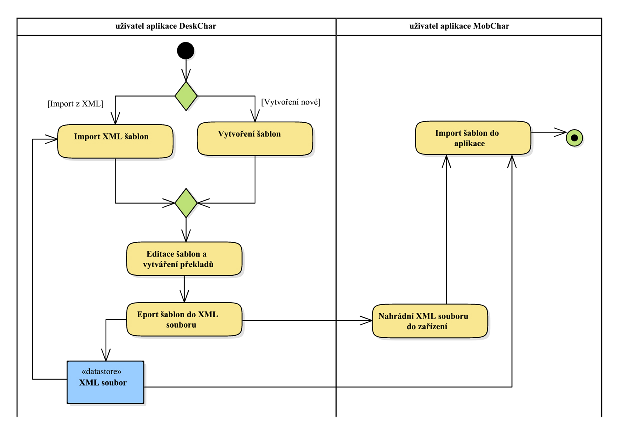
\includegraphics[width=0.8\textwidth]{images/bussiness_sablony}
	\caption[Business proces vytváření šablon]{Model bussines procesů vytváření šablon}\label{fig:bp_sablony}
\end{figure}
Diagram na obrázku \ref{fig:bp_sablony} popisuje základní proces práce se šablonami. Proces popisuje vytváření šablon a následné nahrání do mobilní aplikace. Šablony vytvoříme v~programu nebo případně importujeme z~XML souboru vytvořeném buď aplikací DeskChar nebo například aplikací MobChar. Samozřejmě import a vytváření nových šablon lze kombinovat. Při tomto procesu nevzniká pouze jedna šablona, ale celý soubor šablon, obvykle jednoho typu. Následně jsou provedeny veškeré potřebné úpravy a vytvořené překlady (pokud jsou nějaké zapotřebí). Daná šablona je následně exportována do strukturovaného souboru XML ve~formátu, který podporuje aplikace MobChar. Uživatel mobilní aplikace si vytvořený soubor nahraje do zařízení a následně provede import do aplikace. Nyní je již možné s~novou šablonou pracovat.

\subsection{Vytváření dobrodružství}
\begin{figure}\centering
	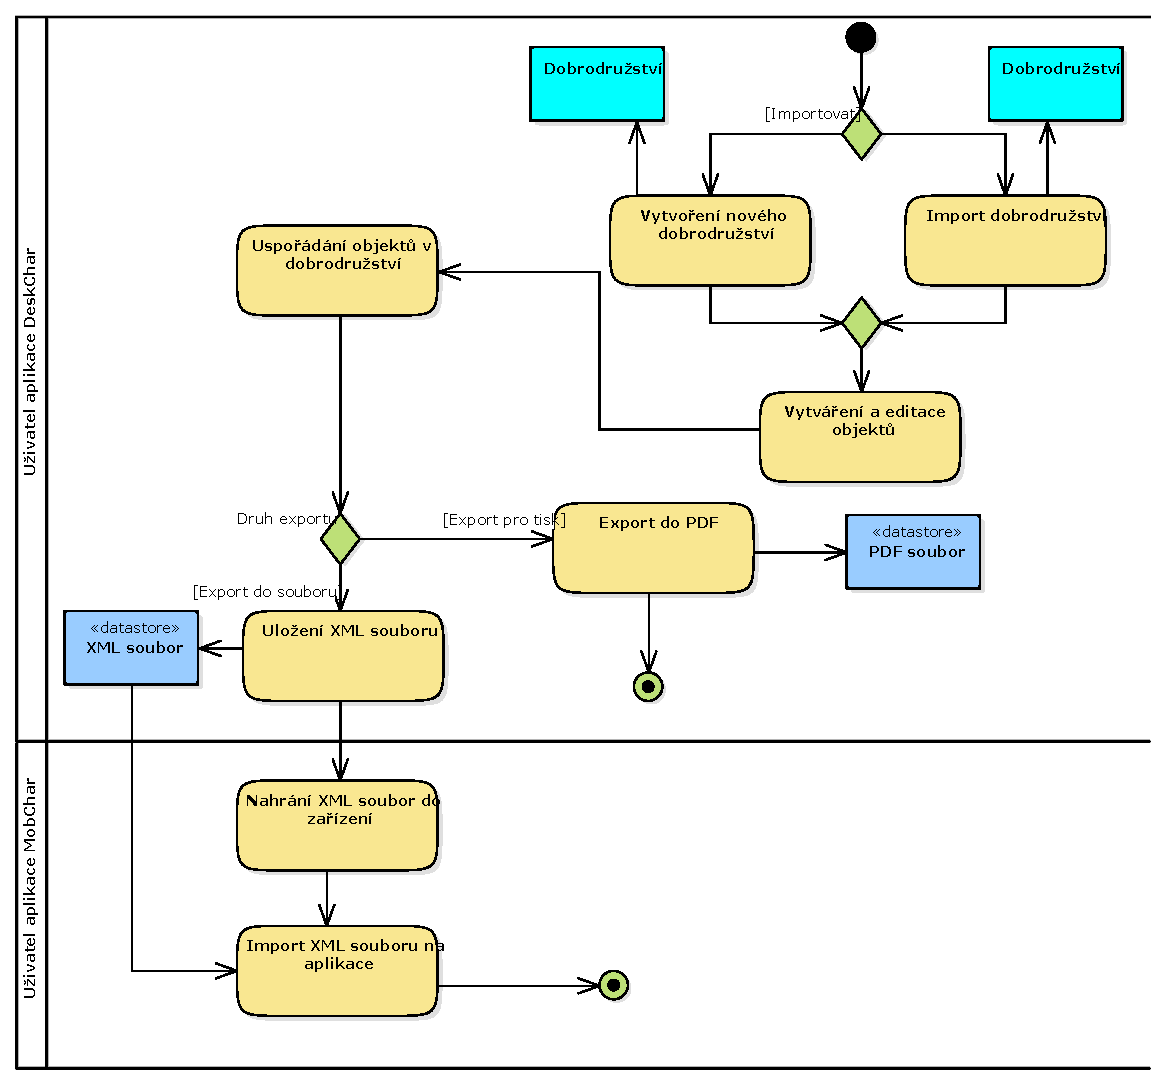
\includegraphics[width=0.8\textwidth]{images/business_dobrodruzstvi}
	\caption[Business proces vytváření dobrodružství]{Model bussines procesů vytváření dobrodružství}\label{fig:bp_dobrodruzsvi}
\end{figure}
Diagram na obrázku \ref{fig:bp_dobrodruzsvi} popisuje proces, při kterém vzniká nové dobrodružství. Objekt dobrodružství se také řadí mezi šablony, protože má velice podobnou funkcionalitu. Protože se jedná o~hlavní šablonu, která v~sobě obsahuje větší počet šablon různých druhů, je proces vytváření dobrodružství popsán více dopodrobna. Na začátku procesu se vytvoří nové dobrodružství nebo se importuje již existující a dále se bude upravovat již stávající hodnoty. V bodě \texttt{Vytváření a editace objektů} se jedná o~bussines proces popsaný v~kapitole \ref{sec:vytvareni_sablon},ve kterém se vytvoří veškeré potřebné objekty, které budou součástí dobrodružství. Veškeré šablony se do dobrodružství přidají a rozřadí se podle potřeby pro větší přehlednost (podle částí dobrodružství, podle typu šablony atd.). Když jsou veškeré úpravy hotové, lze výsledné dobrodružství exportovat. Zde si lze vybrat, zda dobrodružství exportovat pro tisk do formátu HTML nebo pro mobilní aplikaci MobChar ve strukturovaném formátu XML.
\begin{description}

\item[Formát pro tisk] Ze seznamu se vyberou objekty, které budou exportovány (nemusí být exportováno celé dobrodružství naráz) a následně se provede export. Vytvoří se nám přehledný HTML soubor, který je možné následně vytisknout nebo nahrát do zařízení, které umí pracovat s formátem HTML, na což je dostačující obyčejný webový prohlížeč.

\item[Formát pro MobChar] Při exportu do formátu XML se vždy exportuje celé dobrodružství. Nedají se vybrat pouze některé části. Aplikace vytvoří XML soubor. Uživatel následně získaný soubor nahraje do zařízení a importuje ho do aplikace. Takto vytvořené dobrodružství je určené pro mobilní aplikaci MobChar pro Pána jeskyně.

\end{description}

\subsection{Tvorba mapy}
\begin{figure}\centering
	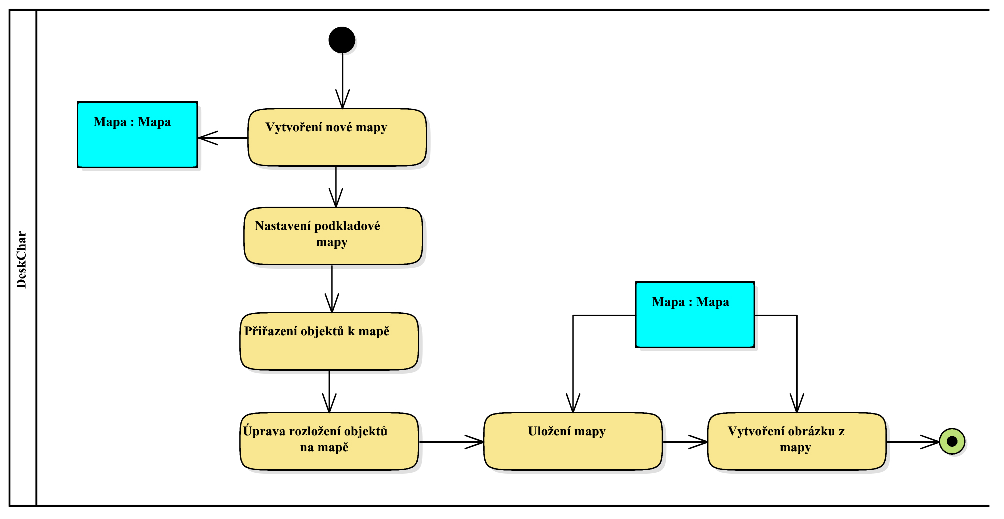
\includegraphics[width=0.8\textwidth]{images/business_mapa}
	\caption[Proces vytváření mapy]{Proces vytváření mapy}\label{fig:bp_mapa}
\end{figure}	
Diagram na obrázku \ref{fig:bp_mapa} popisuje proces vytváření mapy pro dobrodružství. Na začátku se vytvoří nová mapa a nastaví se její základní údaje, což je jméno a popis. V další části se do mapy vloží podkladový obrázek, který bude sloužit jako základ mapy. Tento obrázek se dá kdykoliv změnit, čímž se původní obrázek smaže a nahradí novým. \par

Následuje část, ve které se do mapy přidávají jednotlivé objekty. Vybere se požadovaný objekt a vyplní se u něj jméno a základní popis. Objekt se přidá na mapu. Následně je upravena jeho velikost a umístění na mapě pomocí klasické práce s obrázkem. Tato činnost se opakuje, dokud nejsou všechny potřebné objekty na svém místě. Následuje uložení mapy a rozložení předmětů. Po uložení rozložení automaticky následuje vygenerování nového obrázku z mapy, který se používá při exportu pro mobilní aplikaci.

%% -*-*-*-*-*-*-*-*-*--* Případy užití *-*-*-*-*-*-*-*-*-*-*-*-*-*-*
	\section{Případy užití}	
	\label{part:usecase}
	\begin{figure}\centering
		\includegraphics[width=1\textwidth]{images/pokryti.pdf}
		\caption[Tabulka pokrytí požadavků případy užití]{Tabulka pokrytí požadavků případy užití}
		\label{fig:pokryti}
	\end{figure}
Případy užití popisují jednotlivé způsoby využití aplikace, které uživatel může využívat. Diagram byl rozdělen na tři hlavní části pro větší přehlednost. Na obrázku \ref{fig:pokryti} pak můžeme vidět tabulku pokrytí požadavků případy užití.

\subsection{Práce se šablonami}
	\begin{figure}\centering
		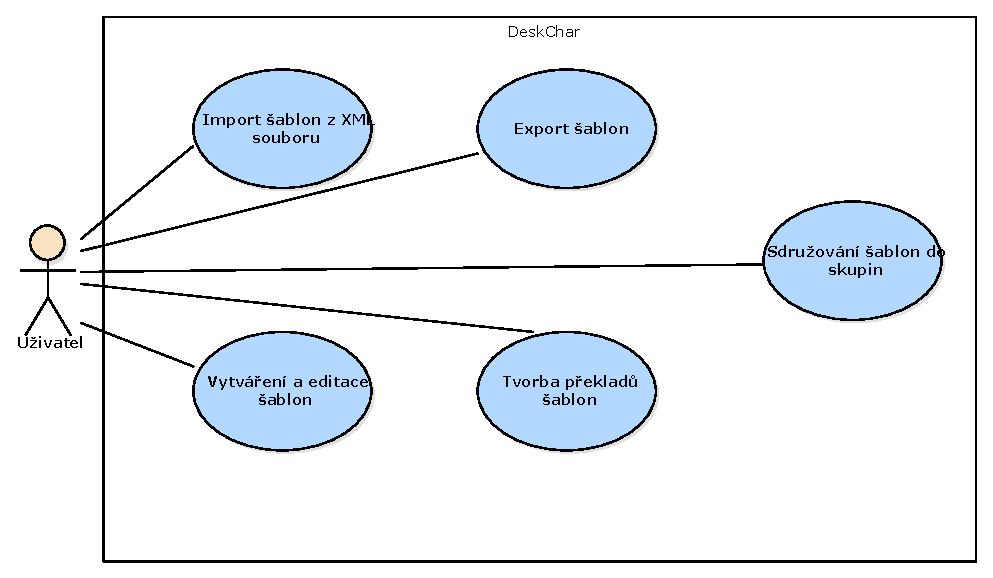
\includegraphics[width=0.8\textwidth]{images/usecase-sablony.pdf}
		\caption[Případy užití pro šablony]{Případy užití pro práci se šablonami}			\label{fig:uc_sablony}
	\end{figure}

Množina případů užití týkající se práce se šablonami namodelovaná na obrázku \ref{fig:uc_sablony} popisuje všechny operace, které je možné se šablonami dělat. Dobrodružství a postavy jsou složené z jednotlivých šablon, které se dají využít i samostatně. Samotné dobrodružství a postavy mají stejný formát jako šablony a navíc mohou obsahovat základní šablony (například postavy mohou mít u sebe zbraně).

\begin{description}
\item[Vytváření a editace šablon] Uživatel si bude moci vytvořit nové šablony nebo editovat stávající. Veškeré parametry, které je možné do šablony zapsat, lze jednoduše upravovat v přehledném formuláři. Uživatel si může vytvořit libovolný počet šablon, které se na základě návazností sdružují do větších celků (dobrodružství, postava).

\item[Import šablon z XML souboru] Program bude umožňovat import šablon ze strukturovaných XML souborů, které vytváří mobilní aplikace MobChar a také samotný program DeskChar. Importované šablony se přidají do databáze a lze s nimi následně provádět stejné činnosti jako s nově vytvořenými. Import z formátu XML je možný pouze pro konkrétní objekt, kde ostatní šablony z XML souboru nejsou využity.

\item[Sdružování šablon do skupin] Veškeré šablony půjde rozřazovat do stromové struktury pro větší přehlednost a jednoduší práci s nimi. Pomocí vytváření složek a jednoduchého drag\&drop systému bude rozřazování velice jednoduché a intuitivní. Díky rozřazení do složek je následná práce se šablonami velice usnadněná, ať už se jedná o hromadný export nebo přiřazování rodičovských šablon.

\item[Export šablon] Veškeré vytvořené šablony lze z aplikace exportovat. K dispozici jsou dva druhy exportu. První možnost je export pro mobilní aplikace MobChar. Aplikace vytvoří strukturované XML soubory, které odpovídají formátu, který používá mobilní aplikace MobChar. Další možností exportu je HTML formát, který slouží pro tisknutí šablon do přehledného almanachu, který umožní využít šablony i hráčům, kteří mobilní aplikaci nemají nebo ji nechtějí použít. 

\item[Tvorba překladů šablon] Ke každé šabloně vytvořené nebo importované do aplikace lze vytvořit neomezený počet překladů. Překlady se vytváří v rámci jedné šablony, pomocí přehledného přepínaní mezi jazyky. Veškeré hodnoty, pro které překlad nemá smysl (číselné hodnoty, povolání, atd.) budou synchronizovány napříč všemi jazyky.
\end{description}

\subsection{Tvorba dobrodružství}
Druhá část případů užití se týká tvorby dobrodružství. Na obrázku \ref{fig:uc_dobrodruzstvi} jsou namodelovány všechny případy užití, které umožňují práci s dobrodružstvím.
	\begin{figure}\centering
		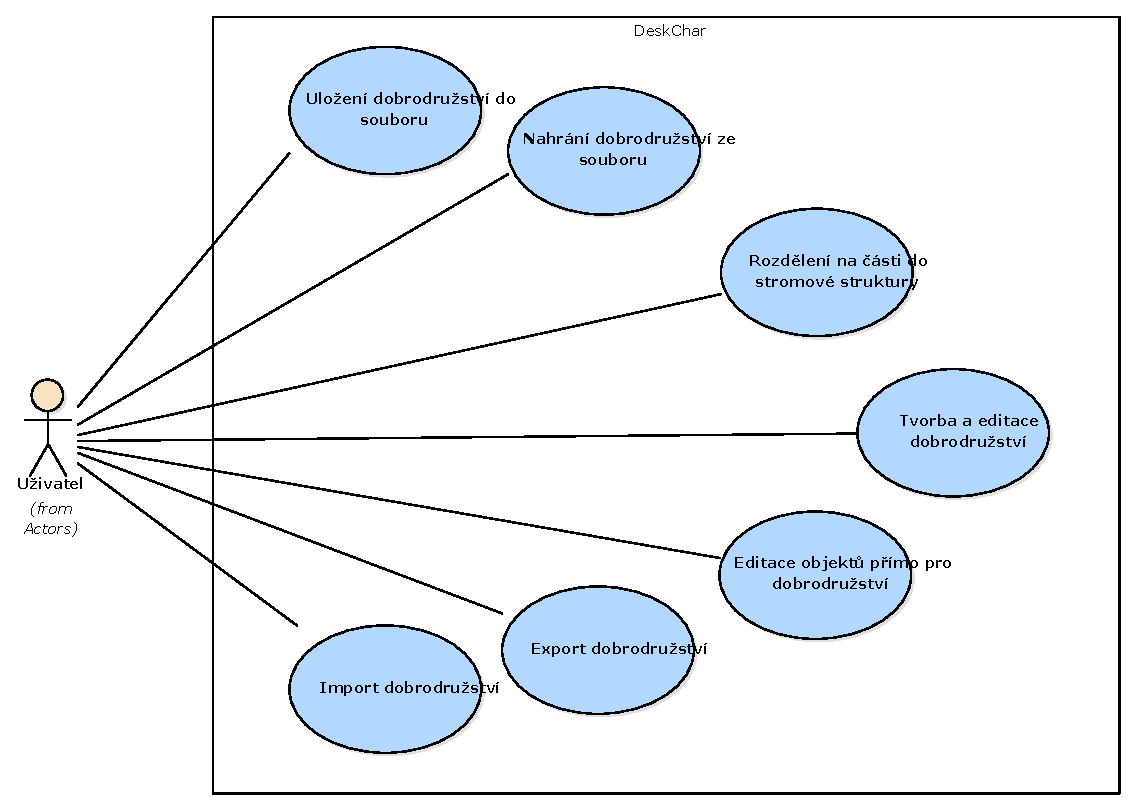
\includegraphics[width=1\textwidth]{images/usecase-dobrodruzstvi.pdf}
		\caption[Případy užití pro dobrodružství]{Případy užití pro práci s dobrodružstvím}			\label{fig:uc_dobrodruzstvi}
	\end{figure}
	
	\begin{description}
		\item[Uložení dobrodružství do souboru]
Celé dobrodružství, včetně veškerých šablon, které se v~aplikaci nachází, je možné uložit do jednoho souboru s~příponou \texttt{.drd}. Tento soubor obsahuje všechny vyplněné údaje šablon a také veškeré obrázky map. V tomto formátu se ukládají i mapy ve formátu, který umožňuje plné obnovení a následnou editaci. 

		\item[Nahrání dobrodružství ze souboru]
V~aplikaci je možné otevřít soubor s příponou \texttt{.drd}, která obsahuje celé uložené dobrodružství včetně všech šablon. Tento formát také umožňuje plné obnovení map, včetně veškerých objektů na mapě. Mapy a celé dobrodružství je nadále možné upravovat. Do aplikace se dá nahrát pouze jeden soubor DRD, všechna ostatní data v aplikaci jsou smazána.
 
		\item[Rozdělení na části do stromové struktury]
		Všechny části dobrodružství je možné rozdělovat do přehledné stromové struktury. Každý objekt má množinu objektů, které může obsahovat. Mimo to se dají vytvářet složky, které mohou obsahovat všechny objekty. Třídění objektů probíhá pomocí systému drag\&drop. Při pokusu o přesunutí objektu na nesprávné místo se struktura stromu nezmění. 
		
		\item[Tvorba a editace dobrodružství]
V aplikaci je možné vytvořit neomezené množství dobrodružství. Dobrodružství se skládají z jednotlivých lokací, které dobrodružství rozdělují na logické celky, a předmětů, kouzel a schopností, které jsou společné pro celé dobrodružství. Do dobrodružství lze přidávat předpřipravené šablony ostatních objektů. 

		\item[Editace objektů přímo pro dobrodružství]
Po přidání objektu ze šablony do dobrodružství se vytvoří nový objekt pomocí hluboké kopie, což znamená úplné zkopírování veškerých dat a vytvoření nového objektu. Tento objekt je pak možné přímo ze záložky dobrodružství editovat a ukládat. Podle druhu objektu se otevře příslušný formulář pro editaci dané šablony.

		\item[Export dobrodružství]
		Celé dobrodružství je možné vyexportovat do strukturovaného formátu XML, který podporuje mobilní aplikace MobChar. K~vyexportovanému dobrodružství se připojí složka resources, ve které se nachází veškeré mapy použité v dobrodružství, které mobilní aplikace umí zobrazit. 
		
		\item[Import dobrodružství]
		Dobrodružství je také možné ze strukturovaného XML souboru importovat. Z~jednoho souboru lze nahrát pouze jedno dobrodružství. Při importu dobrodružství do aplikace se do dobrodružství nepřidají mapy, protože XML soubor v sobě neobsahuje údaje, které by umožňovaly mapu editovat. Do aplikace je možné importovat libovolné množství dobrodružství.
	\end{description}
	
\subsection{Tvorba mapy}
Poslední část případů užití se týká mapy. Na obrázku \ref{fig:uc_mapa} jsou namodelovány všechny případy užití, které aplikace umožňuje.
	\begin{figure}\centering
		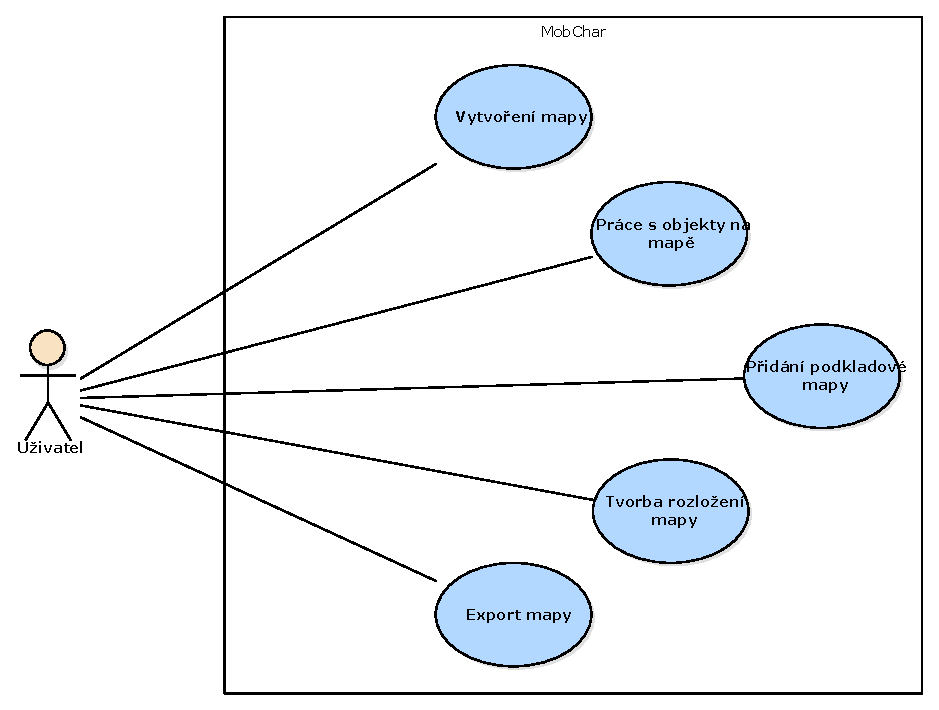
\includegraphics[width=1\textwidth]{images/usecase-mapa.pdf}
		\caption[Případy užití pro mapu]{Případy užití pro práci s mapou}				\label{fig:uc_mapa}
	\end{figure}
	
	\begin{description}
		\item[Vytvoření mapy]
V aplikaci je možné vytvořit libovolné množství map, které se následně dají přiřadit do jednotlivých lokací. Každá mapa má svůj název a základní popis. Mapy je možné jako veškeré objekty rozřazovat do stromové struktury. 

		\item[Práce s objekty na mapě]
Na mapu je možné přidávat jednotlivé objekty. Objekty jsou rozděleny na čtyři základní druhy. Objekt \texttt{monster}, který reprezentuje na mapě nestvůry a všechny postavy. Objekt \texttt{item} reprezentuje na mapě všechny předměty, ať už se jedná o truhlu s pokladem nebo tajné klíče, či nádoby. Další objekt je \texttt{room}, který slouží k popisu místností a lokací. Poslední objekt je \texttt{general}, který zastupuje všechny ostatní objekty na mapě, které je potřeba na mapě zaznamenat. Všem objektům je možné měnit velikost a umístit je na konkrétní místo na mapě.

		\item[Přidání podkladové mapy]
Základním prvkem mapy je podkladový obrázek, který tvoří základní rozložení mapy. Program podporuje základní druhy obrázků .jpg, .gif a .png. Na mapě se může nacházet pouze jeden podkladový obrázek, pokud se na mapě již nějaký nachází a je přidán další, původní obrázek je smazán. Obrázek je zvětšen na velikost okna.

		\item[Úprava mapy]
Každou mapu je možné upravovat. Mapa se ukládá v editovatelném formátu. Všechny objekty se dají z mapy smazat a veškeré hodnoty objektů se dají upravit. Podkladová mapa se dá také kdykoliv upravit.  
		
		\item[Export mapy]
Mapu je možné exportovat do formátu XML nebo do formátu HTML. Formát XML je převážně určen pro mobilní aplikaci MobChar. Soubor XML je vytvořen včetně přiložené složky \texttt{resources}, která obsahuje veškeré vytvořené mapy ve formátu .png. V XML souboru se nachází seznam objektů, které jsou umístěné na mapě včetně jejich čísla, jména a popisu. Tyto údaje využívá mobilní aplikace. Při exportu do formátu HTML se vytvoří stránka, jejíž hlavní část tvoří obrázek s mapou, pod kterou se nachází seznam všech objektů.

	\end{description}
%% -*-*-*-*-*-*-*-*-*--* Doménový model *-*-*-*-*-*-*-*-*-*-*-*-*-*-*
	\section{Doménový model}
Doménový model má za úkol popsat strukturu tříd v aplikaci a jejich vazby mezi nimi. Pro zaznamenání se využívá UML diagram. Diagram nepopisuje jednotlivé funkce tříd ani atributy, které slouží k implementaci tříd, ale zachycuje pouze základní strukturu.

\subsection{Stromová struktura}
\begin{figure}\centering
	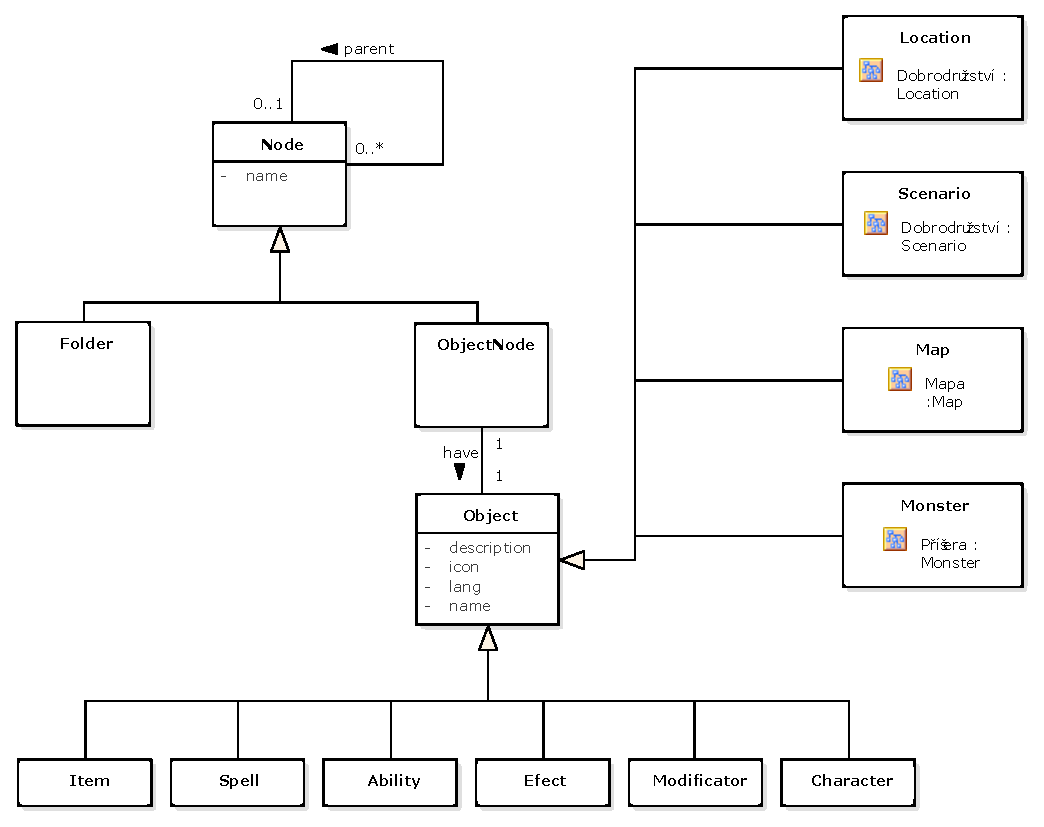
\includegraphics[width=1\textwidth]{images/domain_struktura}
	\caption[Analytický doménový model stromové struktury]{Analytický doménový model stromové struktury}\label{fig:dm_stromova_struktura}
\end{figure}
Diagram na obrázku \ref{fig:dm_stromova_struktura} popisuje strukturu objektů, které slouží pro uchování všech objektů (šablon) a jejich rozřazení do stromové struktury. Veškeré šablony využívají tuto stromovou strukturu. Třída \texttt{Folder} (složka) slouží pouze k rozřazování jednotlivých objektů do skupin. Složka má pouze jméno a může obsahovat libovolný počet složek nebo objektů. \texttt{ObjektNode} pak slouží k uchování šablony samotné. Dolní část objektů na obrázku (\texttt{Item}, \texttt{Spell}, atd.) jsou objekty, které jsou totožné s aplikací MobChar a slouží k uchování šablon pro základní aplikaci a využívají se i v aplikaci pro Pána jeskyně. Pokud vás zajímá podrobnější popis těchto objektů, nahlédněte do bakalářské práce týkající se MobCharu \cite{Weberova_2017}. Oproti tomu, objekty na pravé straně diagramu (\texttt{Map}, \texttt{Scenario}, atd.) jsou objekty, které slouží převážně k vytvoření dobrodružství. Jejich podrobnější popis se nachází dále v textu.\par

Veškeré objekty mohou mít potomky. Systém složek slouží pouze pro přehledné uspořádání. Každý objekt má definované objekty, které může mít jako potomky. Tento systém slouží pro ukládání závislostí, například dobrodružství může obsahovat mnoho lokací, příšer, map a dalších. Některé objekty, jako například kouzla a schopnosti, žádné potomky mít nesmějí. Veškeré vazby mezi objekty jsou zachyceny pouze ve stromové struktuře, aby bylo zabráněno duplikování informací a nebylo nutné tyto údaje synchronizovat.
\subsection{Dobrodružství}
\begin{figure}\centering
	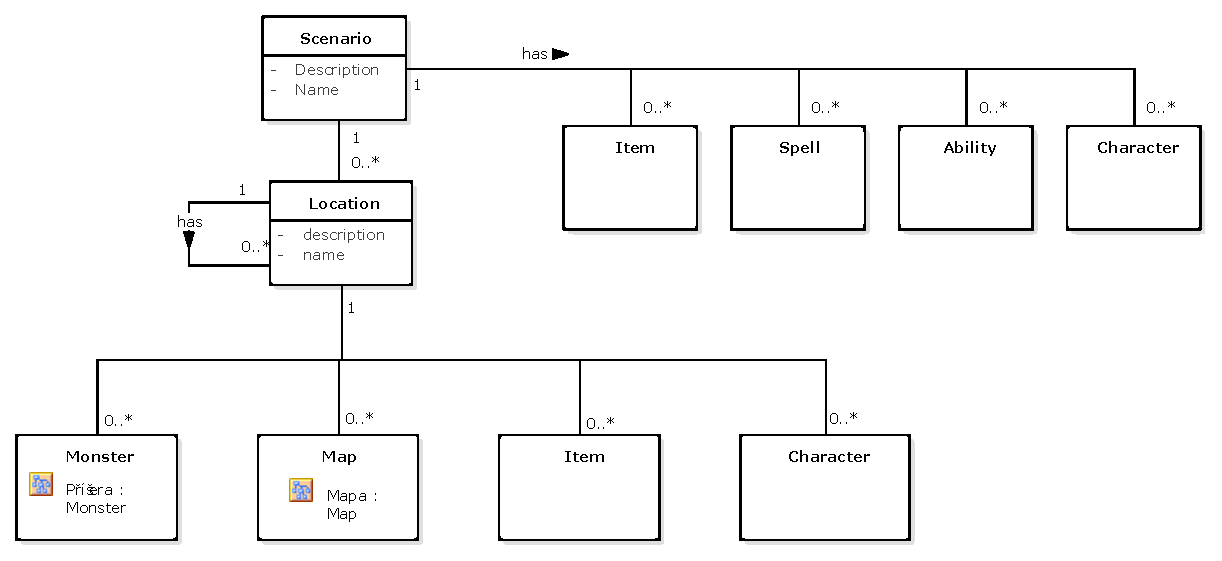
\includegraphics[width=1\textwidth]{images/domain_scenario}
	\caption[Analytický doménový model dobrodružství]{Analytický doménový model dobrodružství}\label{fig:dm_scenario}
\end{figure}
Diagram na obrázku \ref{fig:dm_scenario} popisuje strukturu pro ukládání a práci s~dobrodružstvím. Hlavní třída \texttt{Scenario} je rozdělená do jednotlivých lokací. Pro celé dobrodružství jsou však společné předměty, kouzla, schopnosti a postavy. Předměty, kouzla a schopnosti jsou pro Pána jeskyně, který je nadále poskytuje hráčům, například pokud se hráč má možnost naučit nové kouzlo, nebo získal důležitý předmět pro dobrodružství (elixír, mapa, atd.). Třída \texttt{Character} zde zastupuje postavy hráčů, kteří dané dobrodružství hrají. Jedná se o stejné třídy jako v původní aplikaci MobChar. Pro přesnější popis těchto tříd, je možné nahlédnout do bakalářské práce týkající se aplikace MobChar\cite{Weberova_2017}.\par

Celé dobrodružství je členěné do lokací, které se navíc mohou do sebe zanořovat (lokace může mít pod sebou další lokace). Lokace obsahují příšery, mapy, předměty a postavy. Příšery mají velice podobnou strukturu jako postavy, mohou se naučit schopnosti a kouzla a vlastnit předměty, mají však odlišné atributy, proto jsou od postav odděleny. Jednotlivé mapy mají složitější strukturu, která je popsána níže. Předměty zde znamenají předměty důležité pro tuto lokaci (klíče, věci v bednách a další). Poslední částí jsou postavy, které zde znázorňují postavy, za které nehrají hráči, ale samotný PJ. Jsou to důležité postavy pro dobrodružství, které se nacházejí v dané lokaci. Objekt je stejný jako klasické postavy, ale význam je trochu odlišný.



	\section{Řešení architektury}
\begin{figure}\centering
	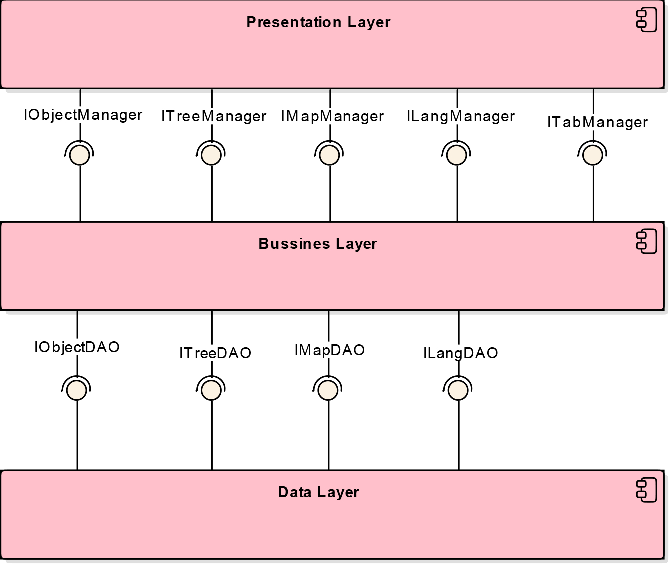
\includegraphics[width=0.8\textwidth]{images/architektura}
	\caption[Model architektury]{Model architektury}\label{fig:architektura}
\end{figure}
Model architektury popisuje formální popis systému, případně jeho detailní plán na úrovni komponent vedoucí k jeho implementaci. Hlavním účelem modelu architektury je popsání hlavních vrstev programu a popis způsobu komunikace mezi nimi.\par

Byla zvolena relaxovaná třívrstvá architektura. Relaxovaná třívrstvá architektura zajišťuje dobrou přehlednost projektu a také snadnou nahraditelnost celé vrstvy programu, například při přechodu na jinou databázi. Veškeré vrstvy mezi sebou komunikují na základě rozhraní definovaného interfaci. Interface je abstraktní třída, ze které musí implementační třída dědit, aby byla zajištěna implementace všech funkcí

\subsection{Vrstvy}
\begin{description}
	\item[Prezentační vrstva] Prezentační vrstva slouží k zobrazení informací pro uživatele. Jedná se o grafickou část celé aplikace. Jejím hlavním úkolem je získávat od uživatele data a naopak uživateli data přehledně zobrazovat. 
	
	\item[Business vrstva] Business vrstva tvoří hlavní spojení mezi datovou a prezentační vrstvou. Business vrstva by se měla starat o veškeré logické operace s objekty, které by správně neměly provádět ani datová ani prezentační vrstva.
	
	\item[Datová vrstva] Hlavním úkolem datové vrstvy je zajistit persistenci dat pro aplikace a také operace s externími soubory. Datová vrstva zajišťuje ukládání dat do databáze a také získávání potřebných dat. Mimo to datová vrstva zajišťuje práci se soubory XML, HTML a drd. 
	
\end{description}



\subsection{Rozhraní}
Mezi vrstvami jsou definovaná rozhraní, která je nutné dodržet. V práci byl využit implementační vzor factory \cite{factory}. Třídy rozhraní poskytují předdefinované funkce, které musí být v implementaci dodrženy. Rozhraní začínají velkým písmenem I, konkrétní implementace daného rozhraní obvykle má stejný název, pouze bez počátečního písmena I.\par

Pro datovou vrstvu se používají takzvané \clqq data access objects\crqq (DAO). Jedná se o třídy, které zajišťují přístup k datům například z databáze a naopak i data ukládají. Pro business vrstvu se využívají takzvané \clqq managery\crqq .\par


\subsubsection*{DAO třídy}
\noindent\textbf{IObjectDAO} v diagramu zastupuje skupinu DAO tříd, které se starají o přístup k datům z databáze a z XML. Na diagramu \ref{fig:architektura} je zobrazen pouze zástupný IObjectDAO, který v implementaci neexistuje a je nahrazen jednotlivými DAO rozhraními (ISpellDAO, IEffectDAO atd.).\\
\\
\textbf{ITreeDAO} se stará o~veškeré ukládání stromové struktury do databáze. \\
\\
\textbf{IMapDAO} se stará o ukládání veškerých dat, která se týkají map. \\
\\
\textbf{ILangDAO} se stará o ukládání jazyků, které jsou v aplikaci použity. Nejedná se o překlady prezentační vrstvy, ale o jazyky vytvořené pro překlady šablon. Rozhraní se nestará o ukládání samotných překladů.\\
\\
\textbf{ISettingsDAO} se stará o ukládání veškerého nastavení aplikace. 

\subsubsection*{Manager třídy}
\textbf{IObjectManager} navazuje na IObjectDAO. Jedná se o skupinu tříd pro veškeré základní objekty (ISpellManager, IAbilityManager, atd.). Rozhraní definuje, jak přijímá data z prezentační vrstvy. Základní funkcionalita spočívá ve zpracování dat z prezentační vrstvy a vytvoření kompletního objektu, se kterým se dále pracuje nebo se pošle na datovou vrstvu pro uložení.\\
\\
\noindent\textbf{ITreeManager} se stará o připravení stromové struktury pro zobrazení. Vytváří z objektů stromovou strukturu a přidává do struktury metadata, která slouží pro zobrazení a práci na prezentační vrstvě.\\
\\
\textbf{IMapManager} se stará o zpracování dat týkající se mapy. Převádí vizuální formu mapy na formu, ve které lze mapu dá uložit do databáze. \\
\\
\textbf{ILangManager} se stará o zpracování dat z prezentační vrstvy týkající se jazyků.\\
\\
\textbf{ISettingsManager} se stará o zpracování dat získaných z widgetu pro nastavení a předání správných dat datové vrstvě.\\
\\
\textbf{ITabManager} se stará o vytváření překladových záložek pro prezentační vrstvu. Toto rozhraní nemá DAO rozhraní, protože veškeré informace které potřebuje, získá přímo z konkrétních IObjectDAO tříd. Jejím hlavním úkolem je zpracování všech překladů jedné šablony a připravení objektů pro uložení.\\





\chapter{Návrh}
Čtvrtá kapitola se věnuje návrhu vytvořené aplikace. Je zde popsán základní model databáze a také popsána struktura hlavních částí formátu XML. Následně je zde pomocí sekvenčního diagramu popsán základní princip zobrazení šablon. V~poslední části této kapitoly je popsán diagram nasazení. Některé nápady a principy návrhu byly čerpány z knížky \textit{Návrhové vzory} \cite{navrhove_vzory}, která se ukázala jako velice užitečná a poučná. \par
Před návrhem je důležité zvolit programovací jazyk, aby některé návrhy byly v tomto jazyku možné a dali se snadno použít. Pro tuto práci byl zvolen programovací jazyk Python. Důvody a popis jazyku Python je popsán v implementační části \ref{programovaci_jazyk}. 
	\section{Model databáze}
	\begin{figure}\centering
	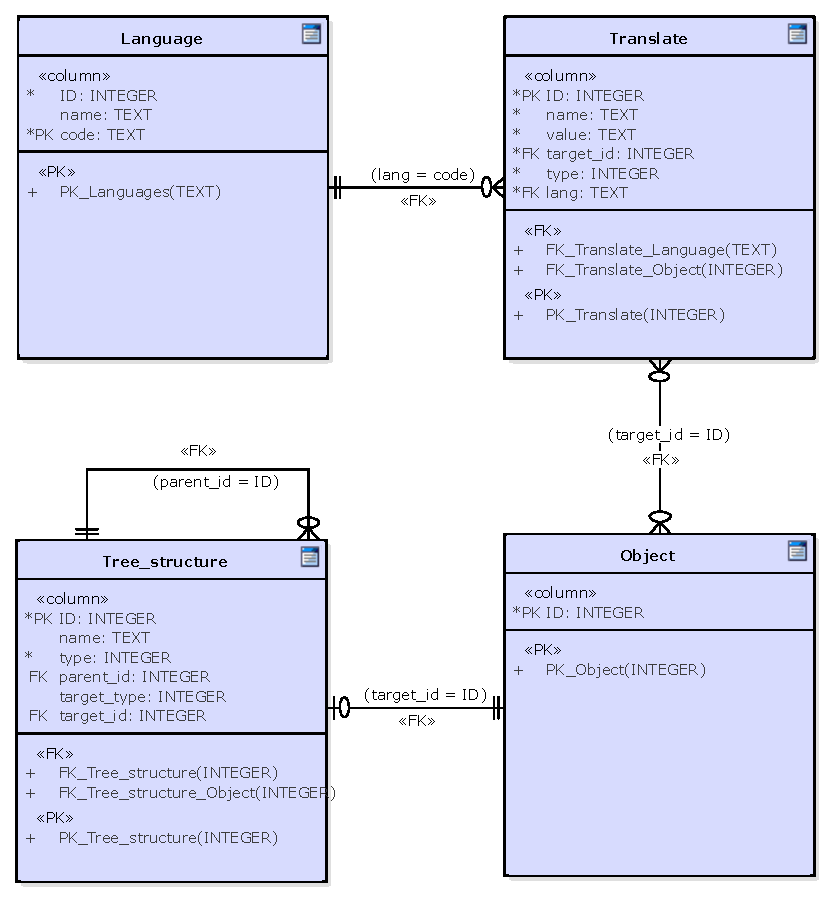
\includegraphics[width=0.8\textwidth]{images/basic_database}
	\caption[Základní model databáze]{Základní model databáze}\label{fig:db_basic}
	\end{figure}
	Pro realizaci aplikace DeskChar byla vybrána databáze \textit{SQLite}, která je jednoduchá a nepotřebuje žádný složitý externí software pro běh. Na druhou stranu zvládá veškeré potřebné operace, jako jsou cizí klíče a kaskádové mazání záznamů. Pro vytváření a práci se stromovou strukturou je kaskádové mazání nedocenitelný pomocník. \par

Diagram na obrázku \ref{fig:db_basic} je zjednodušený pro větší přehlednost. Na diagramu je zachycena základní struktura a princip závislostí v~databázi. Kompletní model databáze se nachází na přiloženém CD.\par

Z důvodu vícejazyčnosti šablon bylo zapotřebí navrhnout strukturu databáze, která dokáže uložit neomezený počet jazykových překladů. Na obrázku \ref{fig:db_basic} můžeme vidět základní strukturu databáze. Údaj o jazyku, ve kterém je daný překlad vytvořen, je uložen v tabulce \texttt{Languages}, který je navázán na tabulku \texttt{Translate} cizím klíčem \texttt{code}. Primárním klíčem každého jazyka je textový kód, který je unikátní. V tabulce \texttt{Translate} pak nalezneme veškeré textové řetězce, které se nacházejí v objektech. Jeden záznam tabulky \texttt{Translate} je přiřazen ke konkrétnímu objektu pomocí dvojice hodnot \texttt{target\_type}, který určuje o jaký objekt (tabulku v databázi) se jedná, a \texttt{target\_id}, který určuje konkrétní záznam v tabulce (ukazuje na primární atribut \texttt{ID} v tabulce). Informace o překladu jsou uloženy ve dvojici hodnot \texttt{name} a \texttt{value}, které slouží jako slovník, jejich jazyk určuje hodnota \texttt{lang}. Takto zvolený návrh databáze umožňuje neomezený počet jazyků a jednoduchou rozšiřitelnost.\par

Druhá část diagramu se týká stromové struktury, která se používá pro všechny objekty v aplikaci. Tabulka \texttt{Tree\_structure} slouží pro zaznamenávání stromové struktury pro veškeré objekty. Do tabulky se ukládají dva druhy uzlů, složky a objekty. Hodnota \texttt{type} určuje, o který druh uzlu se jedná, zda o složku nebo o objekt. Pomocí cizího klíče \texttt{parent\_id} vzniká stromová struktura. Zde se využívá kaskádové mazání - pokud se smaže záznam, který má pod sebou navázané další záznamy pomocí cizího klíče, smažou se tyto záznamy také automaticky v databázi. Tento princip udržuje tabulku konzistentní a nevznikají žádné záznamy, které se již nepoužívají. Každý uzel, který je typu \texttt{object}, je spojeny s konkrétním objektem pomocí dvojice hodnot \texttt{target\_type} a \texttt{target\_id}. Hodnota \texttt{target\_id} určuje tabulku cílového objektu a hodnota \texttt{target\_id} určuje konkrétní záznam v tabulce. V diagramu je tento princip naznačen zjednodušeně, kde tabulka \texttt{Object} zastupuje tabulky všech objektů (\texttt{Spell}, \texttt{Item}, atd.). \par

Poslední problém návrhu databáze se skrýval v návrhu ukládání vazeb mezi jednotlivými objekty. V úvahu připadaly dvě možnosti. První možnost byla zachytit veškeré vazby mezi objekty pomocí tabulek \texttt{relations}, které by obsahovaly pouze dvojici klíčů z obou tabulek. Toto řešení by bylo rychlé a jednoduché na používání, bohužel by se u některých vazeb nedalo použít samostatně. Například u dobrodružství se podřazené objekty mohou sdružovat dále do složek, čehož by se pouze pomocí těchto vazeb nedalo docílit. Musela by se zde navíc využít stromová struktura použitá pro všechny šablony a jejich základní rozřazení, čímž by vznikala duplicitní data. Duplicitní data s sebou nesou dva základní problémy. První z nich je samozřejmě větší množství dat, které je potřebné uložit. V tomto případě by se však nejednalo o drastický nárůst, který by dělal problém. Druhý a závažnější problém se týká aktuálnosti dat. Bylo by zapotřebí udržovat veškeré údaje aktuální a stejné, což by mělo velké nároky na složitost ukládání a zpomalovalo by to některé operace, které je zapotřebí, aby aplikace prováděla okamžitě (například drag\&drop rozřazování). Z těchto důvodů jsem se rozhodl zvolit druhou možnost, kde veškeré vazby mezi objekty jsou uloženy pouze ve stromové struktuře popsané výše. Problém bude vznikat při operacích exportu, kde bude nutné vazbu mezi objekty dohledávat ze stromové struktury. Tyto operace se však neprovádí tak často a není zde velký důraz na okamžitou odezvu. 

	\section{Model XML souborů}
S~doménovým modelem úzce souvisí návrh struktury XML souborů. Struktura těchto souborů je velmi důležitá. Na základě této definované struktury bude probíhat komunikace s~mobilní aplikací MobChar. Formát základních šablon předmětů, kouzel, schopností, efektů, modifikátorů a postav byl převzat z~původní aplikace MobChar pro hráče, aby byla zachována konzistence mezi aplikacemi. Dále se zaměřuji pouze na nově navržené části, což jsou příšery, lokace, mapy a dobrodružství. Pokud vás zajímá struktura základních šablon, nahlédněte do bakalářské práce týkající se aplikace MobChar\cite{Weberova_2017} nebo do přiložené kompletní dokumentace.\par

Struktura XML byla namodelována diagramem, který se normálně využívá pro modelování tříd. Pro tento případ vypovídající hodnota diagramu je dostačující a jasně zadefinovává strukturu XML. Entity v diagramu, které jsou znázorněné žlutou barvou znázorňují již konkrétní XML tag, který uvnitř obsahuje pouze hodnotu a žádné další vnořené tagy. Oproti tomu bílé entity znázorňují pouze obalující tag, který uvnitř obsahuje strukturu dalších tagů. Každá entita v diagramu znázorňuje jeden tag ve výsledném XML dokumentu. Parcialita a kardinalita v diagramu znázorňuje povinnost a případně množství tagů, které se na daném místě v XML souboru mohou objevit. Parcialita vztahu určuje, zda jsou vnořené tagy povinné či nikoliv. V některých případech nemusí být všechny tagy přítomny. Kardinalita určuje, zda na stejné úrovni se těchto tagů může vyskytovat více. Kořenový tag je vždy označen textem  \uv{ROOT} .

\subsection{Dobrodružství}
\begin{figure}\centering
	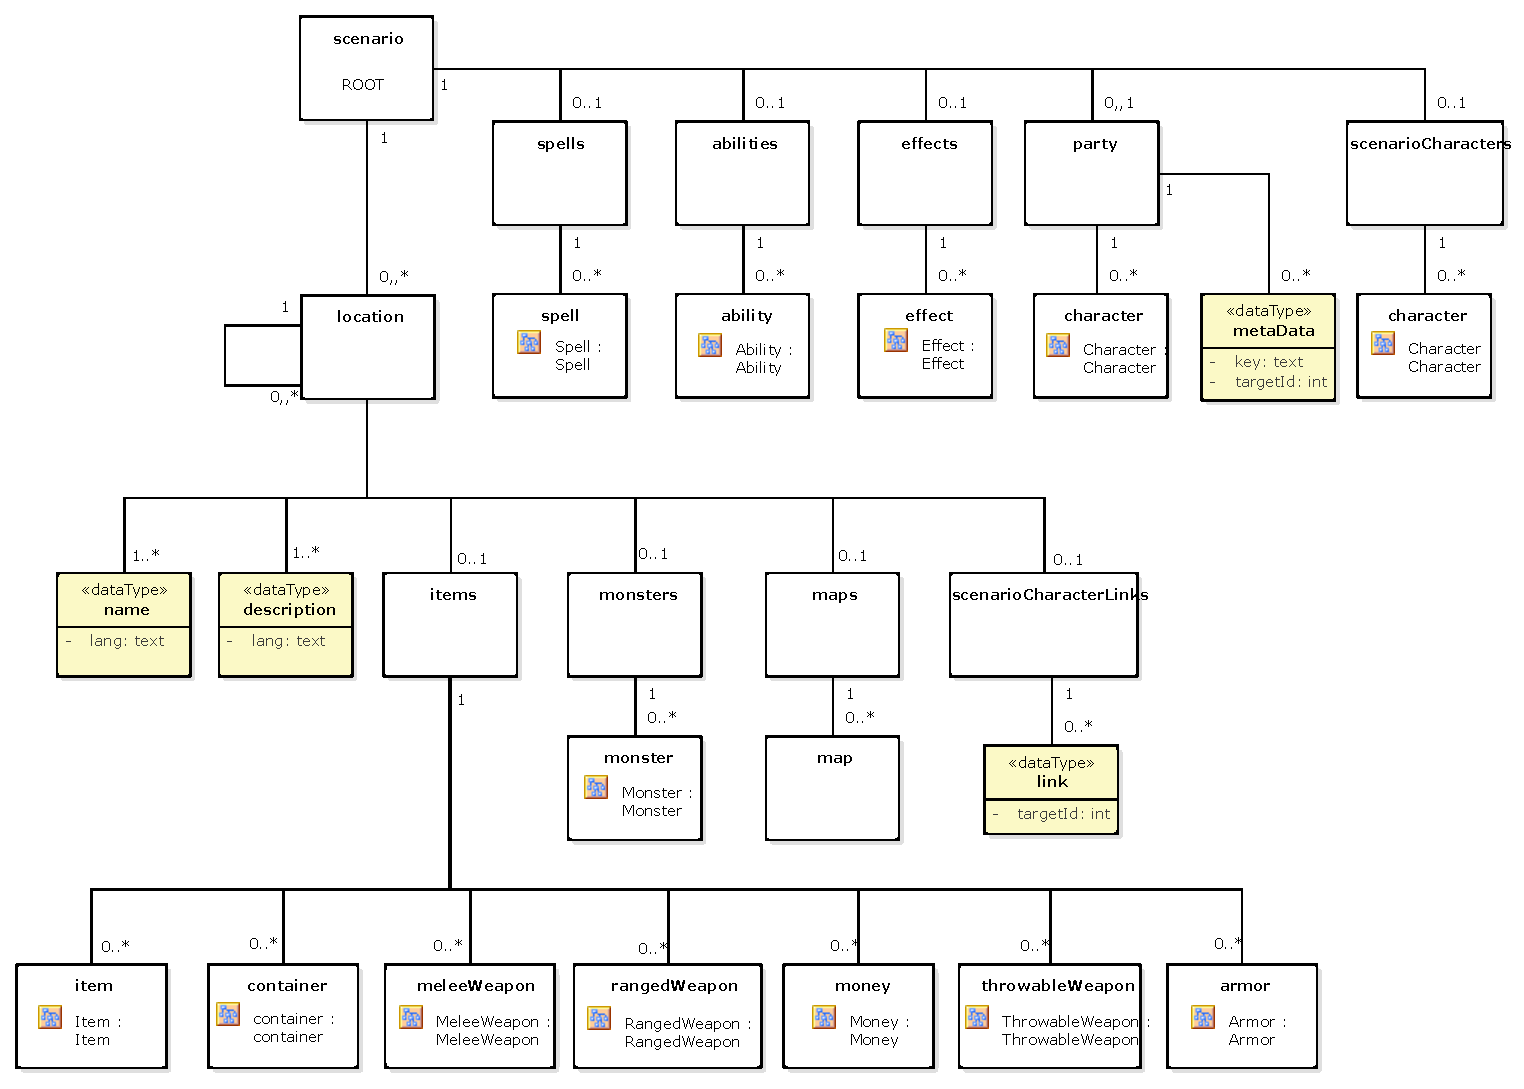
\includegraphics[width=1\textwidth]{images/scenarioXML}
	\caption[Model XML souboru dobrodružství]{Model XML souboru dobrodružství}\label{fig:xml_scenario}
\end{figure}
Struktura XML souboru pro dobrodružství je velice podobná doménovému modelu dobrodružství \ref{fig:dm_scenario}, jak můžeme vidět na obrázku \ref{fig:xml_scenario}. Model XML však má dopodrobna namodelovány veškeré atributy objektů. \par

Obecný princip, který se používá ve všech navržených XML souborech je obalení tagů, které se na dané úrovni mohou vyskytovat vícekrát, rodičovským tagem, jehož jediným cílem je zpřehlednit XML soubor. Tento tag je zpravidla pojmenován jako množné číslo objektů, které obaluje (například pro skupinu tagů \texttt{Spell} se obalující tag jmenuje \texttt{Spells}).

Pro potřeby správného rozeznání předmětů při importu jsou předměty rozděleny do sedmi kategorií, do stejných kategorií, které byly navrženy pro původní aplikaci MobChar. Zde se struktura od původního návrhu šablon lehce změnila. Každá kategorie předmětů již nemá vlastní obalující tag, ale všechny předměty jsou sloučené pod jedním tagem \texttt{items}. \par

Posledním výrazným rozdílem je jiný název pro postavy, které se nacházejí v lokacích. Jelikož se jedná o stejný objekt, se stejnou XML strukturou, ale v rámci celého dobrodružství mají tyto postavy lehce jiný význam, bylo zapotřebí tyto postavy oddělit, aby nebylo nutné se o druhu rozhodovat na základě rodičovského tagu. Proto obalující tag pro postavy, které se nacházejí v lokacích byl pojmenován \texttt{scenarioCharacter}. 

\subsection{Příšery}
\begin{figure}\centering
	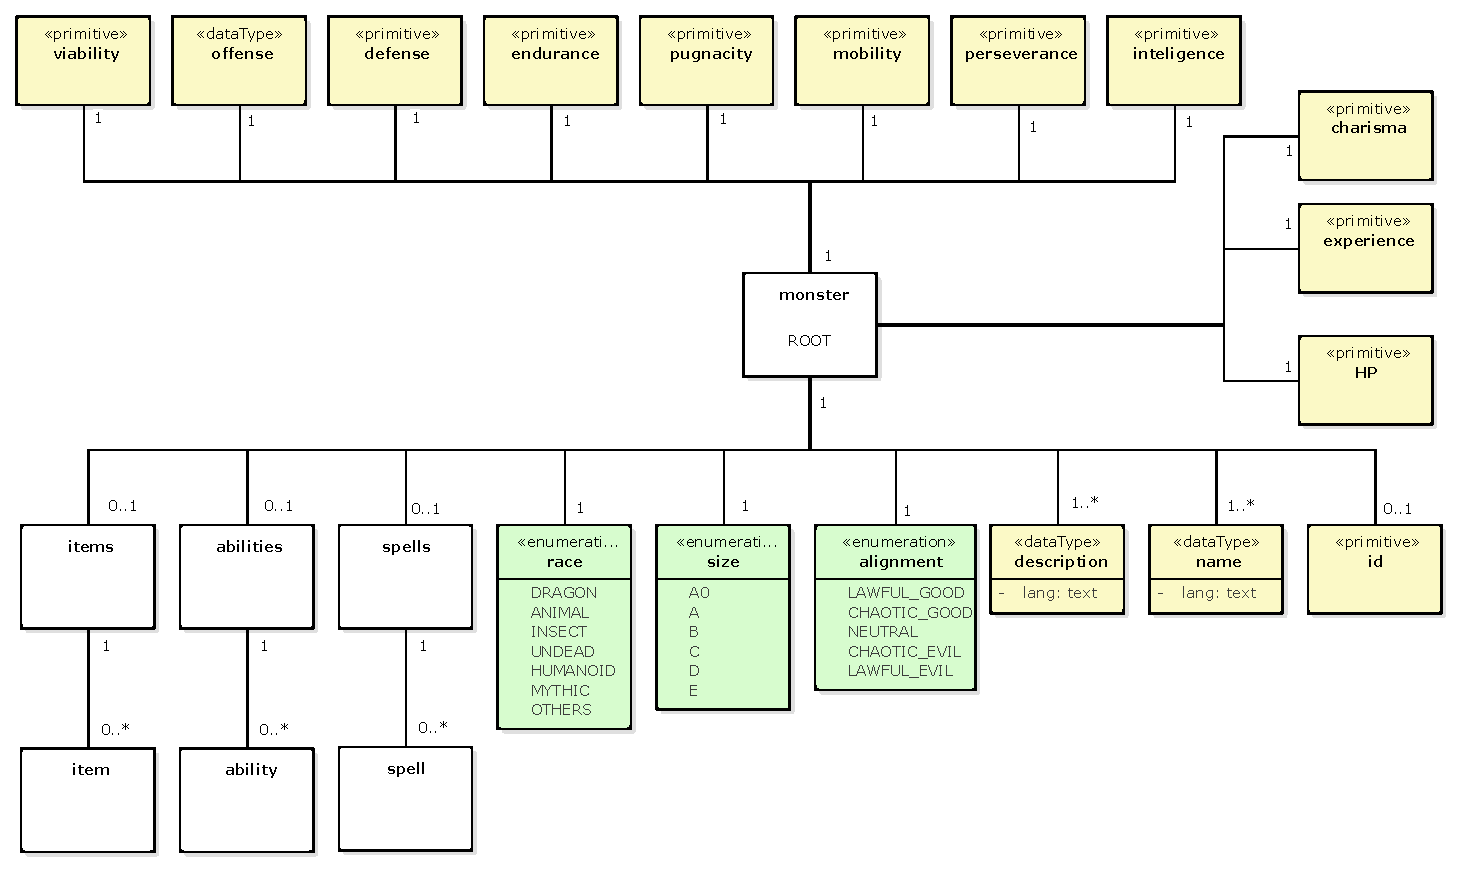
\includegraphics[width=1\textwidth]{images/monsterXML}
	\caption[Model XML souboru příšery]{Model XML souboru příšery}\label{fig:xml_monster}
\end{figure}
Druhá nově zadefinovaná struktura XML souborů se týká příšer. Příšery jsou samozřejmě součástí dobrodružství, jak jste mohli vidět na obrázku \ref{fig:xml_scenario}. Na obrázku \ref{fig:xml_monster} můžeme vidět detailní strukturu souboru. Struktura souboru je podobná struktuře postav, také obsahuje seznam předmětů, schopností a kouzel. Obsahuje tag \texttt{race}, který určuje rasu příšery, ale jedná se o odlišné rasy než pro postavy. Pro určení rasy příšer jsme hledali kompromis, mezi dostatečnou vypovídající hodnotou a konzistencí oproti velkému množství ras, které by se velice rychle stalo nepřehledné. Uživatel si samozřejmě může příšery rozřadit podle libosti na základě stromové struktury nebo případně v popisku příšery. Proto jsme se rozhodli rasy příšer omezit pouze na základních sedm, které můžete vidět na obrázku \ref{fig:xml_monster}. Jedním z hlavních důvodů, proč pro příšery nemohl být použit stejný model jako pro postavy je rozdílná množina základních atributů. Hlavní důvod oddělení příšer od klasických postav byl v rozdílných atributech. Pro počítání výsledku soubojů se používají jiné atributy než u postav. 



	\section{Model komunikace}
	\begin{figure}\centering
	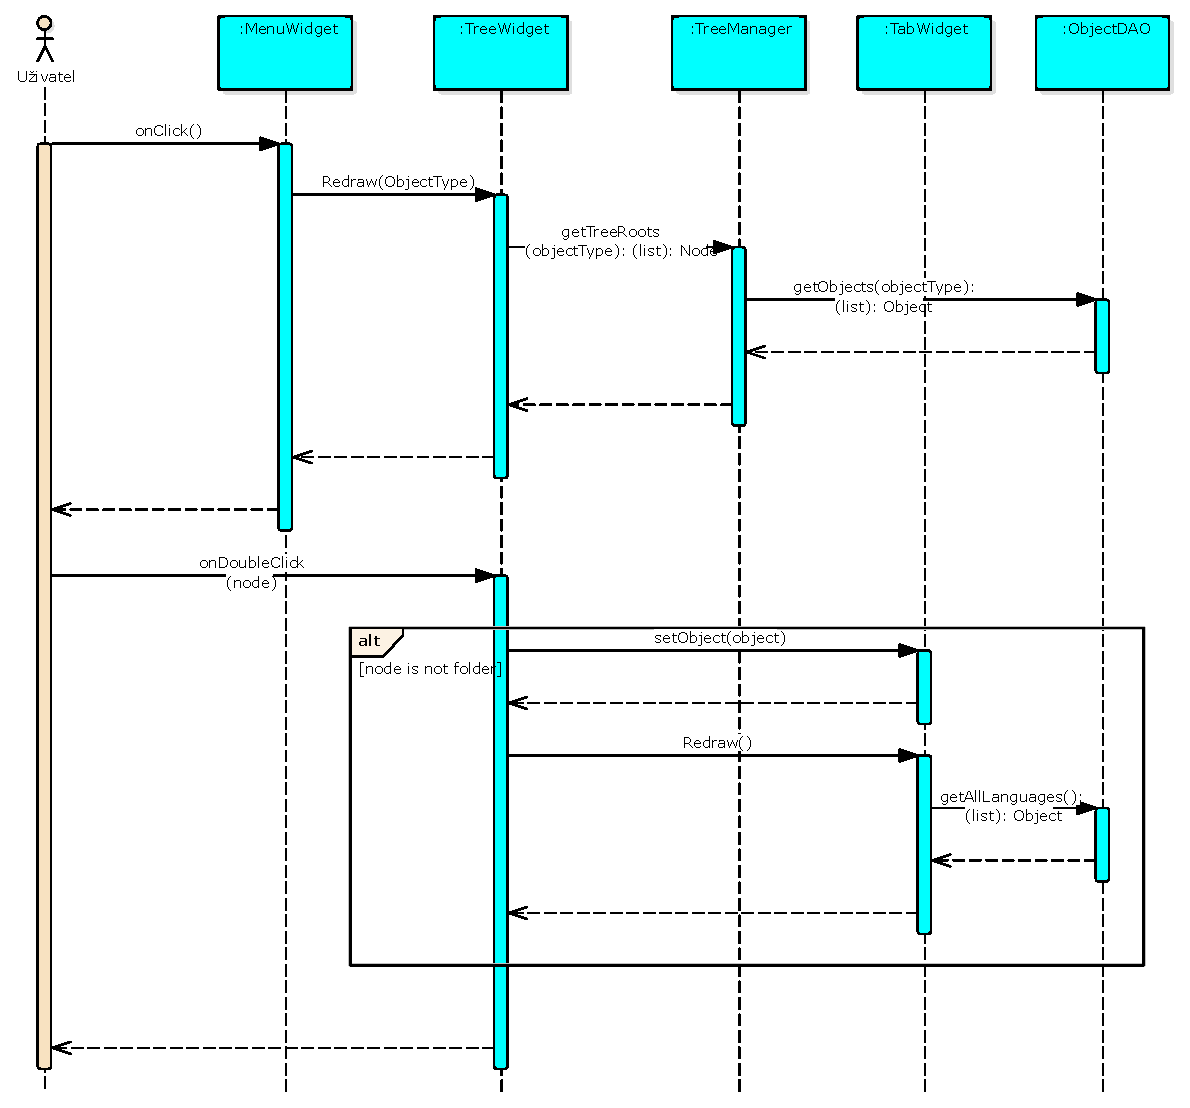
\includegraphics[width=1\textwidth]{images/comunication_main}
	\caption[Model komunikace pro hlavní obrazovku]{Model komunikace pro hlavní obrazovku}\label{fig:comunication_main}
	\end{figure}
Mezi nejčastější operaci prezentační vrstvy patří práce se stromovou strukturou. Na diagramu \ref{fig:comunication_main} můžeme vidět základní dvě činnosti. Vybrání konkrétního typu šablon, které zobrazí stromovou strukturu a zobrazení hlavního widgetu pro vytváření šablon po vybrání konkrétní položky ve stromové struktuře.\par

Uživatel v menu klikne na požadovaný druh šablon. Tím se zavolá funkce \texttt{Redraw}, která má na starosti vykreslení stromové struktury ve widgetu. Potřebná data získá z \texttt{TreeManageru} po zavolání funkce \texttt{getTreeRoots}, která má na starosti, vytvoření kompletního stromu uzlů, přičemž vrací seznam kořenových uzlů. \texttt{TreeWidget} z tohoto listu pomocí rekurze vykreslí celý strom. \texttt{TreeManager} získává data z konkrétní DAO třídy (v diagramu zjednodušena jako \texttt{ObjectDAO}). Objekty navěšené na uzly stromu mohou být různé, takže třída \texttt{TreeManager} volá více různých DAO tříd.\par

Druhá část diagramu se týká vykreslení hlavní části obrazovky, kde se vytváří samotné šablony a jejich překlady. Uživatel ve stromové struktuře dvakrát klikne na nějaký uzel. Pokud se jedná o složku, funkce zavolá pouze rodičovskou funkci \texttt{TreeWidgetu}, což má za následek rozbalení obsahu složky. Pokud se jedná o objekt, zavolá se nad třídou \texttt{TabWidget} funkce \texttt{setObject} s parametrem \texttt{object}. Hned poté se zavolá funkce, která vykreslí všechna data. Data získá na základě nastaveného objektu, který si pamatuje vlastní DAO třídu. Třída vrátí seznam objektů, přičemž se jedná o jednu šablonu, ale ve všech jazycích, ve kterých byla vytvořena. \texttt{TabWidget} následně pro každý jazyk vykreslí jednu záložku, kde se dají hodnoty šablony upravovat nebo případně vytvořit nový překlad pro nový jazyk.
	
	\section{Model nasazení}
	\begin{figure}\centering
	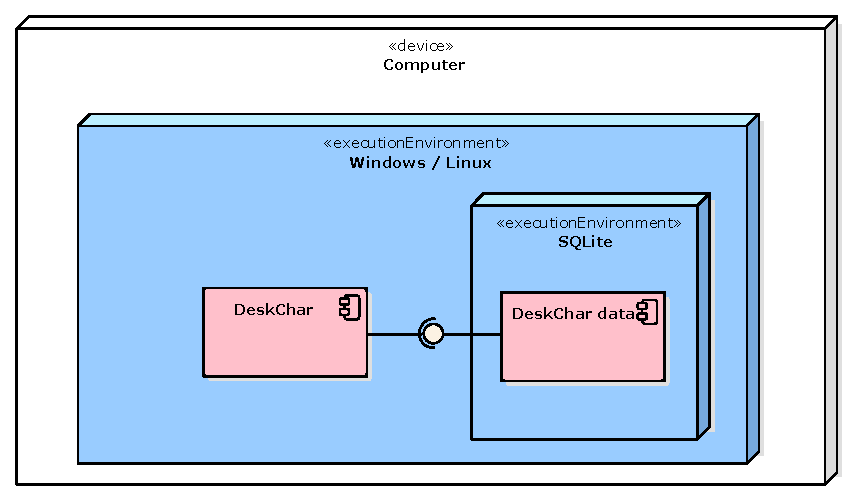
\includegraphics[width=1\textwidth]{images/model_nasazeni}
	\caption[Model nasazení]{Model nasazení}\label{fig:model_nasazeni}
	\end{figure}
Diagram nasazení zobrazuje způsob rozdělení systému na samostatné části a komunikační vazby mezi nimi, čímž definuje architekturu systému. Nalezneme zde veškeré komponenty systému a všechny potřebné části pro běh aplikace.\par

Na obrázku \ref{fig:model_nasazeni} můžeme vidět, že software je určený pro počítače a je funkční pod operačními systémy Windows a Linux (verze operačního systému jsou uvedeny v sekci nefunkční požadavky \ref{sec:nefunkcni_pozadavky}). Aplikace je napsaná v jazyce Python a zabalená do spustitelného balíčku, který nevyžaduje žádné speciální požadavky na systém. Veškeré potřebné knihovny a prostředí má uložené v~balíčku. Databáze SQLite běží v rámci tohoto balíčku také a nepotřebuje žádné dodatečné prostředí.

\chapter{Implementace}
Pátá kapitola se věnuje samotné implementaci programu. Je zde popsaný použitý programovací jazyk a využité knihovny.  Dále jsou zde popsány využité nástroje pro tvorbu celé bakalářské práce. V poslední části jsou popsané problémy, které vznikly při programování aplikace. Některé problémy byly zjištěny na základě testování, které je popsáno v další kapitole.

\section{Použitý programovací jazyk}
\label{programovaci_jazyk}
Jedním z nejdůležitějších rozhodnutí implementace je zvolení programovacího jazyku všech částí. V mnoha případech je programovací jazyk zvolen ještě před začátkem analýzy, což však není ideální. Analýza aplikace by měla být nezávislá na programovacím jazyku. Jelikož se jedná o desktopovou aplikaci, byla zvolena databáze typu SQlite, která je ideální pro práci na jedné stanici. \par

Jako hlavní programovací jazyk pro implementaci byl zvolen Python\cite{python3}. Python je vysokoúrovňový skriptovací netypový programovací jazyk. I když se jedná o převážně scriptovací jazyk, díky velkému množství knihoven je velice snadné v něm psát i rozsáhlé grafické programy. Velká síla jazyka Python se skrývá v tom, že se jedná o netypový programovací jazyk, což v mnoha případech ulehčuje implementaci. \par

Programovací jazyk Python je momentálně vyvíjen ve dvou oddělených a nezávislých větvích a to Python verze 2 a Python verze 3. Pro tuto práci byla zvolena verze 3, která je modernější, většina nových knihoven vzniká právě pro verzi 3 a navíc umožňuje v základu více funkcionalit.

\section{Využité knihovny}
Samotný programovací jazyk je omezen pouze na základní funkce programovacího jazyku. Aby nebylo nutné již existující funkcionality psát znovu, využívají se dodatečné knihovny. Programovací jazyk Python je známý velkým množstvím knihoven, které rozšiřují základní funkcionalitu například o programování grafického rozhraní, matematické výpočty a mnoho dalšího. 
\subsection{Knihovna pro práci s XML}

Velká část programu se týká práce s XML šablonami. Bylo zapotřebí vybrat vhodnou knihovnu, která by veškerou práci co nejvíce usnadnila. Nejsnažší způsob vytváření rozsáhlých XML souborů přímo z objektů je pomocí mapování třídních atributů přímo na atributy v XML objektu. Bohužel taková knihovna, která by tuto funkcionalitu v základu podporovala pro Python neexistuje. Proto byla zvolena knihovna \textit{lxml}\cite{lxml}, která umí základní parsování XML souborů a vytvoření stromového objektu ze získaných dat. Nad touto knihovnou bylo naprogramováno rozšíření pro mapování na objekty, které je blíže popsané dále v textu v sekci implementace.



\subsection{Grafická knihovna}
Pro Python existuje velké množství grafických knihoven. Některé jsou zaměřené na mobilní aplikace, některé hlavně pro webové rozhraní a spoustu se jich také zaměřuje na desktop. Vybrat mezi takovým množstvím knihoven není lehké. Mezi nejznámější patří knihovny \textit{Kivy}, \textit{PyGame}, \textit{TkInter} a \textit{PyQt}. Knihoven pro tvorbu grafického rozhraní existují desítky. Pro rozebrání všech však není v této práci místo a proto jsou zmíněny pouze nejpoužívanější z nich.\par

Knihovna \textit{Kivy} je převážně zaměřená na dotykové displeje. Výsledný vzhled a veškeré widgety jsou pro to přizpůsobeny a ovládání pomocí myši a klávesnice není tak intuitivní jako u~ostatních knihoven.\par

Dalším důležitým kritériem pro výběr knihovny byla aktuálnost a vydávání nových aktualizací a samozřejmě podpora Python verze 3.0.*. Pro knihovnu \textit{TkInter} již dlouho nevychází nové aktualizace. Knihovna je velice jednoduchá a intuitivní, bohužel již několik let není aktuální, proto není příliš vhodná. \par

Knihovna \textit{PyGame}, jak již napovídá její název, se specializuje převážně na tvorbu počítačových her. Má rozsáhlé možnosti animací a herních prvků, které jsou důležité převážně ve hrách. Knihovna neumí vytvářet přehledné grafické rozhraní aplikace, proto byla ze seznamu také vyřazena.\par

Poslední ze čtveřice knihoven je \textit{PyQt}. Knihovna se zaměřuje převážně na tvorbu přehledných grafických rozhraní pro desktopové programy na různé operační systémy, což je přesně to, co je zapotřebí. Navíc má velice moderní vzhled, což bylo jedno z hlavních kritérii pří výběru. Aktualizace k této knihovně jsou vydávány pravidelně a nejnovější a stále aktualizovaná verze PyQt5 je určena pro Python 3. Proto byla tato knihovna zvolena jako nejlepší volba pro tvorbu uživatelského rozhraní. Přesněji byla využita verze knihovny 5.8.
\subsection{Knihovna pro tvorbu HTML almanachů}
\begin{listing}[htbp]
\caption{\label{code:jinja}Ukázka syntaxe šablonovacího systému Jinja}
\begin{minted}[]{jinja}




    <h1> {{ TR['Spell'] }} </h1>
    
        
            
        
    
    


\end{minted}
\end{listing}
Jednou z dalších důležitých funkčností programu je generování HTML almanachů, které budou uzpůsobené pro tisk. Bylo zapotřebí zvolit vhodný šablonovací systém, kterým z předem připravených HTML šablon vytvoří přehledné almanachy, které bude možné prohlížet v~libovolném webovém prohlížeči, kde lze využít křížových odkazů nebo je vytisknout a vzít kamkoliv s sebou. Bylo zapotřebí zvolit vhodný šablonovací systém, který bude umožňovat nejen doplňování proměnných do textu, ale také podmínky a cykly.\par

Mezi nejpoužívanější šablonovací systémy pro Python patří například Mako \cite{mako}, Django templates a Jinja \cite{jinja}. Python podporuje i~velice jednoduchý a základní šablonovací systém nativně. Tento systém je však opravdu velice jednoduchý, nepodporuje žádné podmínky ani cykly a hodí se spíše pro vytváření přehledných výstupů do konzole. Velice rozšířený šablonovací systém je Mako. Jedná se o~výchozí šablonovací systém pro webové frameworky pro Python. Tento nástroj je velice mocný a zvládne velké množství různých funkcí. Bohužel je spíše zaměřený pro tvorbu webových aplikací a práce není příliš přizpůsobená pouze pro tvorbu statických stránek.\par

Jinja a Django templates jsou velice podobné šablonovací systémy, které mají velice podobnou syntaxi. Hlavní nevýhodou Django templates je nutnost instalace celého webového frameworku Django, aby bylo možné šablony zkompilovat a vytvořit výsledný HTML soubor. Proto byl vybrán šablonovací systém Jinja, který je velice populární a existuje pro něj přehledná dokumentace. Je také velice rychlý, takže i~velké množství šablon se vytvoří během chvilky. Na ukázce části šablony \ref{code:jinja} můžete vidět ukázku syntaxe. Jak je vidět, syntaxe je velice podobná syntaxi Pythonu, což velice zjednodušuje práci. Mimo jiné Jinja také podporuje rozdělení šablon do jednotlivých souborů, což velice zpřehledňuje vytváření a editaci šablon.

\subsection{Ostatní knihovny}
Kromě rozšiřujících knihoven byly také použity základní knihovny, které Python poskytuje. Mezi nejpoužívanější patří knihovna \textit{shutil}, která umožňuje snadné kopírování souborů a vytváření složek. Dále knihovna \textit{datetime}, která slouží pro uchování času a exportování do potřebných formátů a také základní knihovny \textit{os} a \textit{sys}, které slouží pro základní práci s operačním systémem, jako je například kontrola existence souborů, nebo správa návratových kódů aplikace.



\section{Použité nástroje}
V této sekci jsou popsány veškeré použité nástroje, které byly použity při vytváření bakalářské práce.

\begin{description}
\item[PyCharm] Pro vývoj kódu aplikace byl využit program PyCharm od české firmy JetBrains. Hlavní výhodou tohoto vývojového prostředí je velké množství editovacích nástrojů, které velice urychlují práci a možnost rozšíření o další funkcionality. Mimo jiné také umožňuje snadné napojení na verzovací systémy jako jsou GIT nebo SVN. Během vývoje aplikace vzniklo několik nových verzí a byl vydán velký update pro rok 2017. Poslední použitá verze byla 2017.1.1.

\item[Enterprise Architect] Tento program slouží pro tvorbu rozsáhlých a přehledných diagramů, které se používají při vytváření analytické dokumentace a při návrhu aplikace. Aplikace umožňuje modelování veškerých UML diagramů, které byly pro práci potřeba. Pro práci byla použita verze 12.0.1215.

\item[GIT] Důležitou částí vývoje je také zálohování a verzování programu. Pro tyto účely byl využit verzovací systém GIT, který umožňuje jednoduchou a přehlednou správu verzí a ukládaní dat na vzdálený server z důvodu zálohování. Pro verzování této práce byl využit GIT pro Windows verze 2.10.0.

\item[MikTex] Celá textová část práce je psaná v jazyku \LaTeX. Pro Windows existuje několik překladačů. Pro tuto práci byl zvolen program MikTex, který umožňuje jednoduchou a rychlou správu rozšiřujících balíčků, čímž eliminuje problém s ručním stahováním potřebných balíčků, což na operačním systému Windows bývá problém. MikTex byl použit ve verzi 2.9.6210.

\item[TexMaker] Program TexMaker je velice přehledný a jednoduchý editor pro Latex. Umožňuje našeptávání syntaxe a také jednoduché zapnutí automatické opravy pro český jazyk, což nepodporují všechny editory. Pro práci byl využit TexMaker verze 4.5.
\end{description}

\section{Adresářová struktura projektu}
\begin{figure}
	\dirtree{%
		.1 business\DTcomment{Složka business vrstvy}.
		.2 managers.
		.3 interface.
		.1 data\DTcomment{Složka datové vrstvy}.
		.2 DAO.
		.3 interface.
		.2 database.
		.2 drdFile.
		.2 html.
		.3 templates.
		.2 xml.
		.3 templates .
		.1 presentation\DTcomment{Složka prezentační vrstvy}.
		.2 dialogs.
		.2 layouts.
		.2 widgets.
		.1 resources\DTcomment{Složka s obrázky a překlady}.
		.2 icons.
		.2 translates.
		.2 maps.
		.1 structure\DTcomment{Složka s definicí hlavních objektů}.
		.2 abilities.
		.2 characters.
		.2 ....
		.1 test\DTcomment{Složka s testy}.
		.2 resources.
	}
	\caption[Adresářová struktura projektu]{Adresářová struktura projektu}
\label{fig:struktura}
\end{figure}
Soubory v projektu jsou logicky rozdělené do složek pro snadnou orientaci v kódu. Na obrázku \ref{fig:struktura} je vyobrazena adresářová struktura celého projektu.  Projekt je rozdělen do šesti hlavních složek.
\begin{description}
\item[business] Složka \texttt{business} obsahuje všechny soubory týkající se business vrstvy. Soubory mají jméno složené z názvu objektu, kterého se třída týká, a slova \texttt{manager}. Složka obsahuje také podsložku \texttt{interface}, ve které se nacházejí veškerá interfaci pro business třídy.

\item[data] Složka \texttt{data} obsahuje veškeré soubory týkající se datové vrstvy. Nachází se zde třídy DAO, které se nacházejí ve složce DAO a jejich název končí stejným klíčovým slovem. Dále jsou zde třídy, které se starají o import a export do formátů XML, HTML a DRD, které jsou rozřazeny do stejnojmenných složek. Ve složce \texttt{database} se nachází třídy pro základní práci s databází.

\item[presentation]Složka \texttt{presenation} obsahuje veškeré soubory, které definují prezentační vrstvu. Soubory jsou logicky rozdělené do složek a hlavní soubory prezentační vrstvy se nachází přímo ve složce \texttt{presentation}. Ve složce \texttt{dialogs} se nachází definice veškerých dialogů a vyskakovacích oken aplikace. Ve složce \texttt{layouts} se nachází definice rozložení formulářů pro editaci veškerých šablon. Složka \texttt{widgets} obsahuje definice hlavních částí uživatelského rozhraní programu.

\item[resources] Ve složce \texttt{resources} se nachází veškeré ikony a překlady pro aplikaci. Také se zde ukládají vygenerované výsledné mapy a zdrojové podkladové mapy.

\item[structure] Ve složce \texttt{structure} se nachází veškeré definice objektových tříd. Soubory jsou rozděleny do logických celků po složkách.

\item[test] Složka \texttt{test} obsahuje definice veškerých testů aplikace. Jméno souborů v této složce musí začínat prefixem test, aby bylo možné testy jednoduše hromadně pouštět. V podsložce \texttt{resources} se nacházejí soubory, které jsou potřeba pro testování, například vzorový XML soubor se šablonami pro porovnání výstupu testů.
\end{description}

\section{Zajímavé části implementace}
V rámci programování aplikace bylo zapotřebí navrhnout mnoho algoritmů a různých principů implementace. V této kapitole jsou popsány dva zajímavé návrhy řešení. První se věnuje nadstavbě knihovny \textit{lxml} a druhý detailně popisuje navržený formát s koncovkou .drd.
	\subsection{Nadstavba knihovny lxml pro mapování objektů}
	\begin{listing}[htbp]
\caption{\label{code:XML}Mapování objektů na XML strukturu}
\begin{minted}[]{python}
class XMLModifier(XMLTemplate):
    ROOT_NAME = 'modifier'
    OBJECT_TYPE = ObjectType.MODIFIER%


    def __init__(self):
        self.id = XElement('id')
        self.valueType = XElement('valueType', ModifierValueTypes)
        self.value = XElement('value')
        self.targetType = XElement('targetType')
        self.valueTargetAttribute = XElement('valueTargetAttribute')


class XMLEffect(XMLTemplate):
    ROOT_NAME = 'effect'
    OBJECT_TYPE = ObjectType.EFFECT


    def __init__(self):
        self.id = XElement('id')
        self.name = XAttribElement('name', 'lang')
        self.description = XAttribElement('description', 'lang')
        self.targetType = XElement('targetType')
        self.modifiers = XInstance('modifiers', XMLModifier)
\end{minted}
\end{listing}
	 V ukázce kódu  \ref{code:XML} můžeme vidět namapování objektů \texttt{Effect} a \texttt{Modifier} a jejich vzájemné provázání pomocí objektu \texttt{XInstance}. \par

Rozšíření obsahuje tři základní třídy, \texttt{XElement}, \texttt{XAttribElement} a \texttt{XInstance}. Každá z těchto tříd reprezentuje jiný typ atributu v objektu. Kombinací těchto tří základních objektů můžeme vytvořit velice komplexní XML soubor. \par

Třída \texttt{XElement} reprezentuje základní atribut, který nemá překlady. V XML se jedná o tag bez atributů a bez vnořených tagů. Jako parametry přijímá název tagu a volitelný atribut \texttt{enum}, díky kterému se hodnota tagu upraví na základě zvolené enum třídy. Posledním volitelný parametr udává, o jaký typ hodnoty tagu se jedná, například pokud je zapotřebí výstup naformátovat jako datum, je třídě předán parametr \texttt{date}. \par

Třída \texttt{XAttribElement} reprezentuje tagy, které mohou navíc obsahovat atributy. Převážně se využívá atribut \texttt{lang}, který slouží pro definici jazyku překladu. Při importu šablony se tyto tagy vyhodnotí jako překladové a vytvoří se slovník hodnot, kde klíče slovníku určují jazyk a jeho hodnoty pak samotný objekt. \par

Poslední třída XInstance reprezentuje vazbu na další mapovací třídu. Jako parametr kromě jména, přijímá instanci cílové mapovací třídy. Objekt se při importu a exportu postará o rekurzivní provolání do dalších tříd. \par

Třída \texttt{XMLTemplate}, ze které všechny mapovací třídy dědí, obsahuje dvě základní funkce, \texttt{import\_xml} a \texttt{create\_xml}. Funkce \texttt{import\_xml} načte XML soubor a vrátí seznam objektů, které se dále načítají do databáze. Jednotlivé objekty jsou navíc rozděleny do slovníku podle jazyků, aby bylo možné importovat vícejazyčné překlady. O proti tomu funkce \texttt{create\_xml} přijímá seznam objektů, ze kterých vytvoří strukturovaný XML soubor. \par

Každá definice XML objektu musí dědit ze třídy \texttt{XMLTemplate} a navíc mít definovaný třídní atribut \texttt{ROOT\_NAME}, který určuje název kořenového tagu a atribut \texttt{OBJECT\_TYPE}, který určuje, o který objekt aplikace se jedná. Dále musí obsahovat třídní funkci \texttt{\_\_init\_\_}, která určí mapování atributů objektu na XML objekty. Princip mapování funguje na základě přiřazení třídního atributu, který definuje název atributu v objektu k mapovací XML třídě. 

	\subsection{Soubor pro ukládání dat v aplikaci}
Jelikož bylo nutné přesunout databázi ze souborového uložení pouze do paměti, z důvodu zrychlení aplikace, bylo zapotřebí navrhnout strukturu souboru pro uložení stavu celé aplikace, ze kterého se veškerá data dají snadno a rychle obnovit. Tento soubor neslouží pouze pro uložení rozpracované práce, ale také například pro sdílení dobrodružství s ostatními uživateli. \par

Důležitá data aplikace se skládají ze dvou částí. První část je obsah databáze, kde jsou uloženy veškeré hodnoty, překlady a struktura všech šablon a objektů. Druhou část tvoří importované podklady pod mapu a uložené hotové mapy. Všechna tato data a soubory je zapotřebí uložit do jednoho souboru, aby se s těmito daty dalo jednoduše pracovat. Jelikož soubor musí obsahovat i potřebné obrázky, není možné využít pouze textový formát ukládání. \par

Pro potřeby aplikace byl navržen nový soubor s tématickou koncovkou \texttt{.drd}. Struktura tohoto souboru je velice jednoduchá. Jedná se o obyčejný zip archiv, kterému je změněna koncovka. V tomto archivu se nachází složka s veškerými obrázky a textový soubor, který v sobě obsahuje veškerá data z databáze. \par

Při vytváření tohoto souboru se vytvoří kopie celé databáze, včetně struktury tabulek. Dále se zkopírují veškeré soubory ze složky \texttt{maps}, kde se nachází pouze používané obrázky map. Z těchto souborů se vytvoří zip archiv, kterému se následně změní koncovka na \texttt{.drd}. Při otevření tohoto souboru se naopak archiv rozbalí do dočasné složky, nakopírují se veškeré mapy na příslušné místo, spustí se SQL script, který vytvoří databázi a dočasné soubory se smažou. \par

Tento systém podporuje pouze ukládání a nahrávání všech dat v aplikaci a neumožňuje částečné spojení dat z více souborů. Pro tyto účely se dá využít export do formátu XML a následný import těchto souborů. 


\section{Vzniklé problémy při implementaci}
\label{problemy_implementace}
Při implementaci vzniklo několik problémů, které se v návrhu nedaly odhalit a bylo zapotřebí některé části návrhu upravit nebo naopak rozšířit. Některé problémy se týkaly samotné implementace, což analýza ani návrh nijak nezachycuje. \par 

Na základě uživatelských testů, které jsou popsány dále, vyšlo najevo, že největší problém aplikace se týkal rychlosti některých operací v aplikaci. Problém rychlosti se týkal převážně importu XML šablon do aplikace a překreslování stromové struktury šablon.

	\subsection{Problém s rychlostí importu z XML souborů}
Na základě následně provedených měření bylo zjištěno, že import velkých dobrodružství mohl trvat až několik desítek vteřin, což pro uživatele může být velmi otravné. Pro odhalení problému bylo provedeno podrobné měření částí kódu, aby byla nalezena problematická část kódu. Z měření bylo jasné, že problém způsobuje rychlost zápisu do databáze, který z důvodu získávání hodnot přiřazené hodnoty \texttt{id} z databáze nemohl být celý transakční, ale musel být rozložen na menší transakce. Hodnota \texttt{ID} je důležitá z důvodu mapování překladů na objekt. Tento problém byl vyřešen změnou umístění databáze. Z původního souboru, který se nacházel na pevném disku, byla celá databáze přesunuta do paměti. Tento přesun bohužel způsobil ztrátu veškerých neuložených dat po ukončení aplikace. \par 

Aby byly ztráty dat eliminovány na minimum bylo současně do aplikace přidáno množství kontrolních dotazů v podobě kontrolních oken, které informují uživatele o případné ztrátě dat. Dále byl také zjednodušen a zrychlen systém ukládání a nahrávání DRD souborů, díky čemuž se při znovuotevření aplikace dají data nahrát velice rychle zpátky. 

	\subsection{Problém s rychlostí překreslování stromové struktury}
Jelikož aplikace umožňuje třídění veškerých šablon do přehledné stromové struktury pomocí jednoduchého drag\&drop systému, je zapotřebí, aby tato akce netrvala příliš dlouho. Jelikož při změně struktury stromu, je zapotřebí překreslit celý obsah widgetu, který zobrazuje stromovou strukturu, je zapotřebí tuto akci velice optimalizovat, protože se provádí velmi často. \par

Při základní implementaci se časová náročnost pohybovala v řádu sekund při velkém množství uzlů ve stromové struktuře, což pro systém drag\&drop je naprosto nepřijatelné. Problém zde byl analyzován do nejmenších detailů, aby bylo dosaženo přijatelné časové náročnosti. Po důkladné analýze vyšlo najevo, že jeden z největších problémů je velikost zobrazovaných ikon u jednotlivých položek. \par

Po zmenšení ikon více jak na jednu pětinu, byla doba překreslování snížena na méně než vteřinu, což již je přijatelná hodnota, ne však ideální. Pro ještě větší urychlení bylo zapotřebí upravit některé principy překreslování. Pokud by bylo nutné dosáhnout ještě lepšího výsledku, bylo by zapotřebí upravit některé principy překreslování stromové struktury a při změně dat nepřekreslovat celý strom, ale pouze jeho změněnou část. Jelikož však časová náročnost vzniká až při velice vysokém počtu elementů ve stromové struktuře, bylo toto řešení problému odsunutu do další verze aplikace. 

	\subsection{Problém s křížovými závislostmi}
Další problém který vznikl, se týká problému křížových závislostí modulů nebo tříd. Jazyk Python je především používaný jako skriptovací jazyk, při kterém se obvykle pracuje pouze v jednom souboru, kde importování jiných souborů není potřeba. Při tvoření velkých projektů, které jsou přehledně rozděleny na velké množství modulů může vznikat problém s křížovými závislostmi. Python pro importování jiných tříd neboli modulů používá dvě syntaxe.

\begin{listing}[htbp]
%\caption{\label{code:import1}První způsob importu}
\begin{minted}[]{python}
import data.database.Database

data.database.Database().select(...)
\end{minted}
\end{listing}

Při tomto druhu importu nevznikají problémy s křížovými závislostmi, bohužel se při každém použití daného modulu nebo dané třídy musí pro její definici použít celá cesta. Při poměrně rozsáhlé adresářové struktuře, která byla využita v tomto projektu, se psaní celých cest stane nepříjemné a také velice nepřehledné. Proto pro takto velké projekty je tento způsob nepoužitelný.

\begin{listing}[htbp]
%\caption{\label{code:import1}První způsob importu}
\begin{minted}[]{python}
from data.database.Database import Database

Database().select(...)
\end{minted}
\end{listing}
O proti tomu pokud použijeme tento druhý způsob, již nemusíme psát celé cesty k třídám, což velice zkrátí zápis. Bohužel pokud nám zde vzniknou křížové závislosti, Python si s tím již neumí poradit. Jediná možnost, jak se tohoto problému vyvarovat, je použití lokálních importů. Jedná se o stejné importy jako v případě jedna nebo dvě, ale importy se nenachází na začátku souboru, jak jsme běžně zvyklí, ale přímo v konkrétní funkci, kde daný modul potřebujeme. V takovém případě Python provede import požadovaného modulu až ve chvíli zavolání funkce a nevznikají problémy s křížovou závislostí. Nicméně z hlediska přehlednosti kódu, by se veškeré importy, pokud je to možné, měly psát na začátek souboru. 


%*-*-*-*-*-*-*-*--*-*-*--*-* Testování *-*-*-*-*-*-*-*-*-*-*-*-*-*-*-*-*-*-*-*-*-*-*-*

\chapter{Testování}
Poslední kapitola se věnuje testování vyvinuté aplikace. Testování aplikace bylo provedeno pomocí jednotkových testů a uživatelských testů. V kapitole je dopodrobna popsán způsob testování a rozebrány testované části. U obou skupin testů je popsán jejich účel, průběh testování a výsledky.
	\section{Jednotkové testy}
Jednotkové testy se zaměřují na testování jedné konkrétní třídy a její funkcionality. Testy by měly fungovat nezávisle na ostatních třídách. Pokud se například testuje funkcionalita databáze, neměly by testy nijak ovlivnit produkční databázi. Unit testy byly rozděleny do 4 skupin po logických celcích. K tvorbě jednotkových testů pro Python se používá knihovna \texttt{unittest}.

		\subsection{Testování databáze}
První skupina testů se věnuje přímému testování operací s databází. 
			\subsubsection*{Účel}
Tato skupina testů má za úkol otestovat třídu \texttt{Database}, která má na starosti základní operace s databází. Testují se základní operace jako jsou \texttt{SELECT}, \texttt{CREATE}, \texttt{DELETE} nebo \texttt{INSERT}. Testování probíhá na oddělené databázi, aby nedošlo k poškození aplikační databáze. 			

			\subsubsection*{Výsledky}
Tato skupina testů byla velice nápomocná při odhalování rychlostních problémů celé aplikace. Při spuštění testů je možné vidět i dobu, za kterou se jednotlivé testy provedly, což napomohlo k nalezení nejpomalejší části práce s databází a následné přesunutí databáze do paměti.

		\subsection{Testování DAO tříd}
Další skupina testů se zabývá testováním důležitých DAO tříd. Některé třídy nejsou testované, protože je nelze testovat samostatně.
			\subsubsection*{Účel}
Hlavním účelem této skupiny testů je odhalení chyb při vytváření objektů z databáze a ukládání objektů do databáze. V testech se testují základní operace všech DAO tříd, což jsou \texttt{create}, \texttt{insert}, \texttt{update} a \texttt{delete}. Pro každou DAO třídu se provede několik operací a výsledné objekty se porovnávají, zda jsou správně vytvořené, případně data v databázi upravená. Testy se provádí na stejné struktuře databáze, na jaké běží aplikace, ale z důvodu neovlivnění dat aplikace běží v jiné databázi.
			
			\subsubsection*{Výsledky}
Na základě testování DAO tříd bylo odhaleno mnoho chyb při mapování dat na objekty. Převážně se jednalo o špatné přiřazování hodnot do objektu. Takto odhalené chyby by se bez těchto testů velmi špatně odhalovaly.			

		\subsection{Testování importu a exportu XML}
Třetí skupina testů se zabývá kontrolou správné práce s XML soubory.

			\subsubsection*{Účel}
Hlavním účelem těchto testů je kontrola správné práce s XML soubory, jak při importu do aplikace, tak při exportu z aplikace. \par

Při testování XML souborů do aplikace se využívají připravené šablony. V aplikaci se spustí import dat pro danou šablonu a kontrolují se výsledné objekty, které při importu vzniknou. Data se kontrolují pouze na základě objektu, neukládají se do databáze. Kontrolují se veškeré hodnoty všech objektů, kromě hodnoty \texttt{id}, která se může měnit. Samozřejmě se také kontroluje správné zanořování objektů. \par

Při exportu objektů do XML souboru se kontroluje struktura výsledného XML souboru. Aby bylo možné výsledné soubory porovnávat, vzorový soubor a výstupní soubor jsou patřičně seřazeny podle abecedy. Kontroluje se přítomnost všech potřebných tagů, které aplikace MobChar vyžaduje a také jejich hodnota.

			\subsubsection*{Výsledky}
Na základě testování práce s XML soubory bylo odhaleno množství chyb, které by se daly snadno odhalit při uživatelských testech, ale při tomto testování je snadnější odhalit konkrétní chybu a není potřeba zdlouhavě komunikovat s mobilní aplikací. Díky těmto testům bylo výrazně sníženo množství chyb, které se musely opravovat na základě uživatelských testů. 

	\subsection{Testování DRD souboru}
Poslední skupina testů testuje vytváření DRD souboru a jeho správný obsah.

			\subsubsection*{Účel}
Hlavním účelem těchto testů je kontrola vytváření a správného obsahu souboru DRD. Testy využívají připravené databáze, ze které se soubor vytvoří. Soubor se vytvoří do dočasné složky, kde se také rozbalí. Zkontrolují se veškerá přítomná data, která jsou tvořena z databázového souboru a také složky s mapami. Po skončení testů se veškeré dočasné soubory smažou, aby neovlivnily další spuštění testů.

			\subsubsection*{Výsledek}
Na základě těchto testů máme zajištěno, snadné odhalení potencionální chyby, pokud bychom změnili strukturu adresářů nebo provedli jiný větší zásah do aplikace.

\section{Uživatelské testování}
Další možností testování aplikace jsou uživatelské testy. Uživatelské testy mají simulovat praktické využití aplikace. Na rozdíl od jednotkových testů, kde veškerou funkcionalitu testuje počítač, uživatelské testy provádějí lidé. Uživatelské testy se provádějí na základě připravených scénářů. \par

Pro případy testování se zpravidla připravuje speciální verze programu, která veškeré chování zaznamenává, aby bylo možné snadněji odhalit chyby. Testovací uživatel dostane scénáře, které mu říkají, jaké činnosti má v aplikaci vyzkoušet. Pokud vše funguje jak je uvedeno ve scénáři, uživatel ohodnotí test jako splněný, v opačném případě test označí jako nesplněný a do komentáře napíše problém, který vznikl. Uživatel také může do komentáře napsat i připomínky v případě, že scénář proběhl v pořádku, ale některé věci se nechovají jak by očekával. 

\subsection{Účel}
Hlavním účelem uživatelských testů, které byly vytvořeny pro aplikaci, bylo otestování veškerých scénářů, které jsou popsány v kapitole \ref{part:usecase}. Pokud veškeré scénáře uživatelkým testováním projdou, můžeme na základě tabulky, která popisuje pokrytí požadavky, rozhodnout, že aplikace splňuje veškeré požadavky, které byly na začátku stanoveny. 

\subsection{Průběh}
Jelikož aplikace DeskChar nevzniká jako samostatná aplikace, mělo by uživatelské testování probíhat v rámci celého balíčku. Velká část funkcionality aplikace se týká exportování XML souborů pro mobilní aplikace, které bez těchto aplikací není možné vyzkoušet. Pro testovací uživatele byl vytvořen testovací balíček, který obsahuje veškeré potřebné instalační soubory pro nainstalování celého balíčku aplikací, krátký popis instalace a veškeré testovací scénáře. \par

Z důvodu velkého množství testovacích scénářů pro všechny aplikace jsou v této práci uvedeny pouze scénáře, týkající se aplikace DeskChar. Ostatní scénáře jsou podrobněji popsány v pracích Matěje Sháněla \cite{Shanel_2017} a Šárky Weberové \cite{Weberova_2017}. 

\subsubsection{Práce se šablonami}
První z testovacích scénářů se týká vytváření šablon pro aplikaci MobChar. Tyto šablony se pak dále využívají také při tvorbě dobrodružství. Uživatel testuje základní práci se šablonami v aplikaci. Postup je totožný pro všechny druhy šablon, proto je popsán pouze scénář pro jeden druh šablon. \par

Uživatel si vytvoří libovolné množství předmětů. U každého předmětu vyplní všechny potřebné údaje a šablony uloží. K některým šablonám vytvoří alespoň další dva překlady. Následně některé šablony smaže. Zkontroluje zda všechny údaje jsou uložené správně, překlady jsou správně uložené a všechny číselné hodnoty se mění naráz na všech záložkách. \par

Pokud vše funguje jak má, testovací uživatel předmětu přidá další objekty, které je možné pod šablony přidat. V případě předmětů se jedná o efekty nebo jiné předměty. Šablony efektů si uživatel vytvoří v záložce efekty stejným postupem, jako vytvářel předměty. Předmětům přidá libovolné množství vnořených efektů nebo předmětů. Následně vyzkouší vytvořené efekty přesunout k jiným předmětům pomocí drag\&drop. \par 

Poslední část scénáře se týká vytvoření adresářové struktury. Testovací uživatel si vytvoří alespoň 3 adresáře, které do sebe vnoří a následně do těchto složek přesune předměty a v některých složkách vytvoří nové předměty. Nakonec uživatel přesune složku včetně obsažených předmětů do kořene stromové struktury. Testovací uživatel zkontroluje, zda se veškeré operace se stromovou strukturou provedly správně. Pokud ano, scénář testující práci se šablonami zde končí úspěchem. 

\subsubsection{Vytváření mapy}
Další scénář se týká vytváření mapy a operace s mapou.  Testovací uživatel se přepne do záložky \texttt{Mapa}. V adresářové struktuře vytvoří novou mapu, vyplní název mapy a dvojklikem se přepne na její editaci. Pomocí ikony \texttt{Přidat podkladovou mapu} vybere soubor, který obsahuje libovolný obrázek. Tento obrázek by měl mít rysy mapy, aby přidávání objektů na mapu mělo smysl. Následně zkusí přidat nový podkladový obrázek, přičemž starý obrázek je tímto nahrazen. \par

Testovací uživatel dále na mapu přidá libovolné množství dalších objektů. Pro každý objekt vybere jeho typ a vyplní základní údaje objektu. Objekt se vytvoří na mapě. Uživatel následně objekt zvětší nebo zmenší podle potřeby a přesune na potřebné místo. Pokud se jedná o větší mapu, uživatel může využít funkcí na přiblížení a oddálení pro lepší práci s mapou. Po přidání několika objektů také některé předměty smaže. Následně mapu uloží a zkontroluje, zda celá mapa zůstala ve stejném stavu a všechny údaje jsou správně uloženy. Pokud vše souhlasí, testovací scénář zde končí úspěchem. 

\subsubsection{Vytváření dobrodružství}
Další scénář navazuje na předchozí scénáře, protože využívá vytvořené šablony a mapy v předchozích scénářích. Pokud je testování provedeno samostatně, je zapotřebí vytvořit alespoň nějaké šablony a mapy podle předchozích scénářů. Testovací uživatel vytvoří nové dobrodružství. Do dobrodružství přidá libovolné množství předmětů, lokací, kouzel, schopností a postav. Všechny tyto objekty může libovolně roztřídit do složek pro větší přehlednost. Některé objekty zedituje přímo v záložce dobrodružství pomocí dvojkliku na daný objekt ve stromové struktuře. Pokud všechny možné operace se provedou správně, testovací scénář zde úspěšně končí.

\subsubsection{Práce s formátem XML}
Tento scénář převážně testuje funkčnost komunikace s mobilními aplikacemi MobChar, jak s balíčkem pro hráče, tak s balíčkem pro Pána jeskyně. Pro potřeby testování se opět využívají vytvořené šablony a objekty z předešlých scénářů. Pokud testování probíhá samostatně, je nejdříve zapotřebí vytvořit dostatečné množství šablon a objektů, nejlépe alespoň dvě od každého druhu, podle předchozích scénářů. \par

První část scénáře se zaměřuje na komunikaci s hráčskou aplikací. Uživatel postupně pro každý druh šablon provede stejnou operaci a také vyexportuje alespoň jednu postavu. Přepne se do sekce pro danou šablonu a zvolí možnost exportovat. Ve stromové struktuře se objeví zaškrtávací políčka, pomocí kterých vybere požadované šablony pro export. Po dokončení výběru uživatel vybere možnost \texttt{Export XML}, kde v otevřeném okně vybere cílový soubor, do kterého se šablony vyexportují. \par

Výsledné soubory nahraje do zařízení, ve kterém se nachází nainstalovaná aplikace MobChar, na patřičná místa. Následuje testovací scénář, který se týká aplikace MobChar, který je detailně popsán v práci Šárky Weberové \cite{Weberova_2017}. Po provedení příslušného testování mobilní aplikace vytvoří soubory XML, které je možné zpět do naší aplikace nahrát. \par

Uživatel se přepne do záložky, která se týká šablon, které chce importovat. Pokud se v XML souboru nachází i šablony jiného druhu, tyto šablony jsou vynechány. Uživatel vybere tlačítko \texttt{Importovat} a v novém okně vybere zdrojový soubor. Aplikace provede import všech šablon správného typu a zobrazí nově vytvořené šablony. Uživatel zkontroluje, zda obsahují všechny údaje, které aplikaci byly předány pomocí XML souboru. Uživatel provede tuto operaci pro všechny druhy šablon a také pro postavu. V poslední části vyzkouší importovat poškozený XML soubor, přičemž by aplikace měla vytvořit chybovou hlášku, která informuje o nezdařeném importu. \par

Velice podobný průběh má scénář, který testuje komunikaci s aplikací pro Pány jeskyně. Testovací uživatel se přepne do záložky \texttt{Dobrodružství} a vybere tlačítko export. Zvolí požadované dobrodružství a vybere možnost \texttt{Export XML}. V novém okně vybere cílový soubor, kam se výsledek exportu uloží. Výsledný XML soubor nahraje do mobilního zařízení, kde se nachází nainstalovaná aplikace MobChar. \par

Dále probíhá testování na základě scénářů definovaných v práci Matěje Sháněla \cite{Shanel_2017}. Po provedení veškerých testů týkajících se dobrodružství, aplikace vytvoří nový XML soubor, který je možné zpět nahrát do aplikace DeskChar. Testovací uživatel výsledný soubor nakopíruje zpět na testovací zařízení. \par

V aplikaci v záložce \texttt{Dobrodružství} vybere možnost \texttt{Importovat} a zvolí zdrojový soubor. Po provedení úspěšného importu, se v záložce zobrazí nové dobrodružství. Veškeré části dobrodružství by měly být na správných místech a obsahovat všechny předané údaje. Import dobrodružství neumožňuje vytvoření map, proto se mapy do dobrodružství nevytvoří. Uživatel zkontroluje správnost všech údajů a celé struktury. Pokud vše souhlasí testovací scénář zde končí úspěchem.

\subsubsection{Práce s formátem DRD}
Krátký testovací scénář se týká testování práce se soubory s koncovkou .drd. Uživatel si v aplikaci vytvoří libovolné množství šablon a objektů. V menu zvolí možnost \texttt{Uložit}. Pokud aplikace nebyla ze souboru DRD otevřena, objeví se nové okno pro zadání cíle pro uložení. Po zvolení cílového souboru a potvrzení jsou data do souboru uložena. Následně uživatel upraví některé šablony v aplikaci. Následně pokud opět zvolí možnost \texttt{Uložit}, aplikace by se již neměla na umístění zeptat. Je možné však data uložit na jiné umístnění pomocí možnosti \texttt{Uložit jako}. \par

Uživatel aplikaci zavře a znovu otevře. Všechna data z aplikace jsou smazána. Uživatel zvolí možnost \texttt{Otevřít} a v novém okně vybere dříve vytvořený soubor. Aplikace data načte a znovu vytvoří všechny uložené šablony a objekty. Při ukládání do formátu DRD je možné zachovat i mapy, tudíž při otevření souboru se obnoví i veškeré uložené mapy. Testovací uživatel zkontroluje přítomnost a správnost všech dat. Pokud vše souhlasí, končí zde testovací scénář úspěchem.

\subsubsection{Vytváření HTML almanachů}
Poslední testovací scénář se týká vytváření HTML almanachů. Uživatel opět potřebuje mít vytvořené šablony a objekty z předchozích scénářů. Testování se provádí na všech šablonách a objektech. Scénáře jsou totožné pro všechny záložky. \par

Testovací uživatel se přepne do konkrétní záložky a vybere možnost \texttt{Exportovat}. V zobrazených zaškrtávacích políčkách vybere objekty, které chce exportovat. Následně vybere možnost \texttt{Export HTML} a v novém okně vybere cíl, kam se výsledné soubory uloží. Aplikace na dané místo vygeneruje potřebné soubory. \par

Uživatel otevře soubor \texttt{index.html}. Soubor zkontroluje, že obsahuje všechny zvolené šablony a u každé všechny vyplněné parametry. Hlavním cílem tohoto scénáře je zjistit, zda jsou výsledné almanachy přehledné a dobře uzpůsobené pro tisk. Pokud uživatel uzná, že všechny údaje jsou uvedené a almanach je dostatečně přehledný, testovací scénář zde končí úspěchem. 

\subsection{Výsledky}
Pro uživatelské testy bylo domluveno několik Pánů jeskyně a také dvě kompletní skupiny hráčů. Všem testovacím uživatelům byl předán stejný testovací balíček, včetně veškerých potřebných scénářů. Testovací uživatelé si scénáře prošli a poslali zpět odezvu. Odezva se týkala všech testovaných aplikací. V této práci jsou uvedeny pouze odezvy, týkající se aplikace MobChar. Ostatní jsou k nahlédnutí v práci Matěje Sháněla\cite{Shanel_2017} a v práci Šárky Weberové \cite{Weberova_2017}. \par

Uživatelé, především Páni jeskyně, si aplikaci DeskChar vyzkoušeli a dopodrobna vyzkoušeli všechny funkcionality a prošli všechny vytvořené scénáře. \par

Dle testovacích uživatelů byl největší problém aplikace její rychlost. Některé činnosti trvaly příliš dlouho, což velice zdržovalo práci s aplikací. Z tohoto důvodu byl věnován čas na vylepšení časové náročnosti některých operací, který je popsán v kapitole implementace \ref{problemy_implementace}. \par

Dále uživatelé narazili na drobné chyby týkající se správného nastavování hodnot u šablon modifikátorů. Tyto problémy byly na základě odezvy opraveny. \par

Bez ohledu na nalezené drobné chyby byli všichni testovací uživatelé s aplikací spokojeni. Někteří uživatelé poslali návrh na nové funkce, které by aplikace mohla umožňovat. Tyto funkcionality byli zaevidovány, avšak v této práci již nebudou realizovány. 

% --------------------------------------------Conclusion--------------------------------------
\begin{conclusion}
Cílem této práce bylo vytvořit desktopovou aplikaci DeskChar pro všechny hráče Dračího doupěte v souladu se standardy softwarového inženýrství. \par

V první fázi vývoje aplikace byla vytvořena analýza již existujících aplikací, se kterými výsledná aplikace spolupracuje. Byly analyzovány všechny požadavky na aplikaci a vytvořeny scénáře užívání. Na základě této analýzy vznikl podrobný návrh realizace. Dopodrobna byl popsán návrh tříd, databáze a architektury celého programu. \par

Na základě analýzy a návrhu byl program implementován, včetně veškeré dokumentace a popisu tříd. Následně pomocí jednotkových a uživatelských testů byla ověřena funkcionalita celé aplikace a splnění všech analyzovaných požadavků. Po dokončení celé implementace vznikla k aplikaci uživatelská příručka, která budoucím uživatelům usnadní práci s aplikací. Uživatelská příručka je k dispozici na přiloženém CD. \par

Vytvořením aplikace podle standardů softwarového inženýrství a dodáním plné dokumentace a uživatelské příručky bylo splněno zadání bakalářské práce. \par

Vzniklá aplikace je pouze ve verzi 1.0 a má velký potenciál pro zlepšování. Hlavní směr vývoje pro verzi 2.0 by se měl týkat mapy. Ve verzi 1.0 je editor mapy pouze základní a aplikace zde nabízí velký prostor pro zlepšení. V aktuální verzi jsou možné pouze základní operace s podkladovou mapu. Aplikace by mohla obsahovat vlastní propracovaný editor mapy, kde by se celé mapy dali vytvářet. Dále na podmět testovacích uživatelů, by bylo příjemné do aplikace přidat další mechanismy jako například ochočená zvířata postav.

\end{conclusion}

\bibliographystyle{resources/csn690}
\bibliography{resources/mybibliographyfile}

\appendix

\chapter{Seznam použitých zkratek}
% \printglossaries
\begin{description}
	\item[bash] Born again shell
	\item[DAO] Data access object
	\item[DeskChar] Desktop character
	\item[DrD] Dračí doupě
	\item[enum] Enumeration
	\item[exe] Executable
	\item[HTML] Hypertext Markup Language
	\item[MobChar] Mobile character
	\item[PJ] Pán jeskyně
	\item[UML] Unified Modeling Language
	\item[RPG] Role-playing game
	\item[XML] Extensible Markup Language
\end{description}

 

\chapter{Obsah přiloženého CD/USB}

%upravte podle skutecnosti

\begin{figure}
	\dirtree{%
		.1 readme.txt\DTcomment{stručný popis obsahu CD}.
		.1 doc\DTcomment{dokumentace}.
			.2 model.eap\DTcomment{soubor veškeré modelové dokumentace}.
			.2 UserGuide.pdf\DTcomment{uživatelská příručka}.
		.1 exe\DTcomment{adresář se spustitelnou formou implementace}.
			.2 Windows\DTcomment{spustitelná verze pro Windows}.
			.2 Linux\DTcomment{spustitelná verze pro Linux}.
		.1 src.
			.2 impl\DTcomment{zdrojové kódy implementace}.
			.2 thesis\DTcomment{zdrojová forma práce ve formátu \LaTeX}.
		.1 text\DTcomment{text práce}.
			.2 thesis.pdf\DTcomment{text práce ve formátu PDF}.
			.2 thesis.ps\DTcomment{text práce ve formátu PS}.
	}
\end{figure}

\end{document}
